\documentclass[10pt,a4paper]{article}
\usepackage[T1]{fontenc}
\usepackage[utf8]{inputenc}
\usepackage{lmodern,graphicx,booktabs,longtable,array,amsmath,amssymb,float}
\usepackage[margin=18mm]{geometry}
\usepackage[numbers,sort&compress]{natbib}
\usepackage[hyphens]{url}
\usepackage[hidelinks]{hyperref}
\IfFileExists{microtype.sty}{\usepackage{microtype}}{}
\IfFileExists{caption.sty}{\usepackage[font=small,labelfont=bf]{caption}}{}
\setlength{\parskip}{4pt}
\setlength{\parindent}{0pt}
\setlength{\emergencystretch}{3em}
\setlength{\textfloatsep}{12pt}
\setlength{\intextsep}{12pt}
\setlength{\abovecaptionskip}{6pt}
\renewcommand{\topfraction}{.92}
\renewcommand{\bottomfraction}{.88}
\renewcommand{\textfraction}{.06}
\renewcommand{\floatpagefraction}{.82}
\widowpenalty=10000
\clubpenalty=10000
\makeatletter
\setlength{\@fptop}{0pt}
\makeatother
\newcommand{\figref}[1]{Fig.~\ref{fig:#1}}
\title{Complete figure book: clinical course, serum markers and EASI estimation}
\author{}
\date{}
\begin{document}
\maketitle
This review copy contains the five main figures followed by all 41 supplementary figures. Captions specify populations, uncertainty and what each comparison can establish. Complete numerical results are supplied as CSV source tables.
\clearpage
\renewcommand{\thefigure}{1}
\begin{figure}[p]
\centering
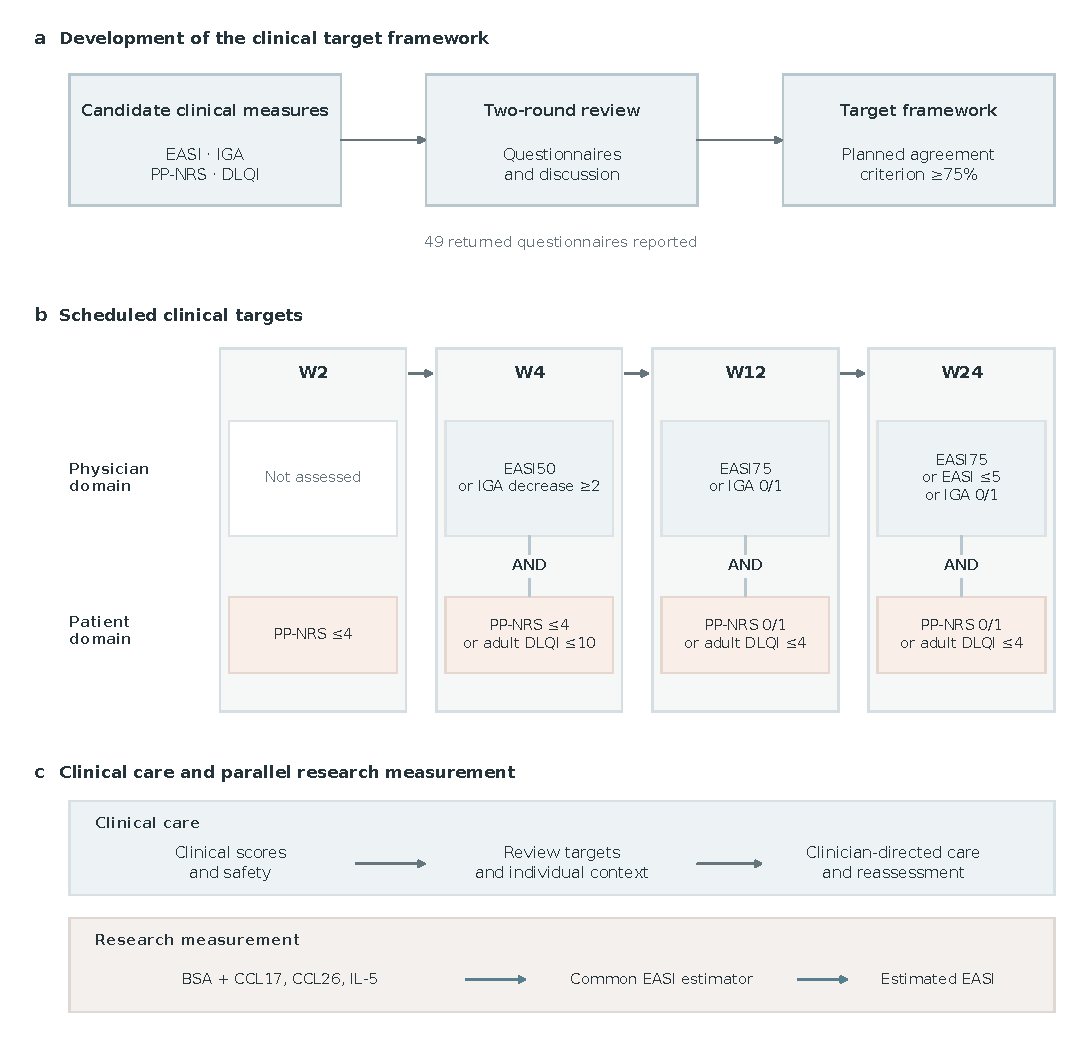
\includegraphics[width=\linewidth,height=.76\textheight,keepaspectratio]{figures/Figure1.pdf}
\caption{\textbf{Source framework, clinical targets and the research readout.} a, The project development summary describes candidate measures, a two-round questionnaire procedure and a planned $\geq$75\% agreement criterion, and reports 49 returned questionnaires. Original ballots and round-specific agreement results are unavailable; this is not a newly verified consensus experiment. b, The operational target schedule follows the source framework; milestone positions are schematic rather than time-scaled. EASI50/75 denotes at least 50\%/75\% improvement from positive observed baseline EASI. IGA decrease $\geq$2 is change from baseline; 0/1 denotes an observed grade or score of 0 or 1. OR applies within a domain and AND across domains. W2 is an itch-only target, not a combined physician-patient target. Adult DLQI requires age $\geq$18. Missing components use three-valued logic; adult DLQI is unknown below age 18. The IGA instrument and approved, implemented framework version require confirmation; these are exploratory recorded-score targets. c, Clinical assessment supports clinician-directed management. The BSA-serum readout is a parallel research addition, with clinical decision use untested. It does not replace examination, symptoms, quality of life or safety review. The cohort does not test framework effectiveness. Detailed definitions and provenance are provided in the Supplementary Methods.}\label{fig:Figure1}
\end{figure}
\clearpage
\renewcommand{\thefigure}{2}
\begin{figure}[p]
\centering
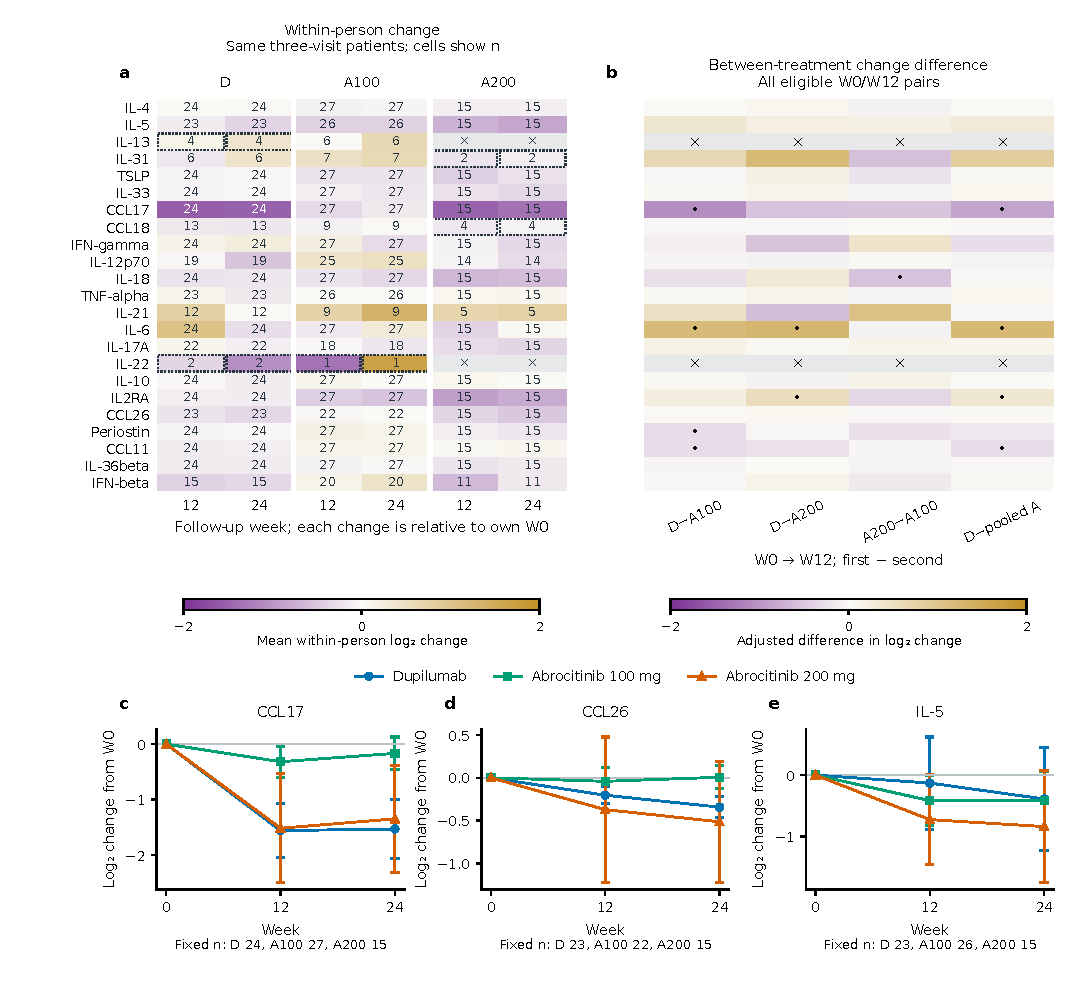
\includegraphics[width=\linewidth,height=.76\textheight,keepaspectratio]{figures/Figure2.pdf}
\caption{\textbf{Clinical course, response depth and target attainment.} a--c, Observed EASI, peak-pruritus numerical rating scale (PP-NRS) and adult Dermatology Life Quality Index (DLQI) medians with interquartile bands by initial treatment. Adult DLQI requires age $\geq$18. d--f, Observed EASI50/75/90 response rates at W4/W12/W24, with Wilson 95\% confidence intervals; response requires positive observed baseline EASI. Counts are in D/A100/A200 order, aligned to actual visits except the separately headed PP-NRS visit table. Lines describe available-case summaries, which need not retain the same patients over time. g, Observed stage-specific target rates with Wilson intervals and achieved/evaluable counts. W2 uses PP-NRS $\leq$4; later combined targets require a physician and a patient criterion, as defined in Fig. 1. Stage criteria differ, so these points are not joined. Missing outcomes remain unknown rather than observed failures. h, EASI differences from the common-reference generalized-overlap-weighted model, adjusted for baseline EASI, age, sex, BMI and centre, with patient-cluster-robust 95\% confidence intervals. Negative values favour the first named group for lower EASI; colour distinguishes W12/W24. D, dupilumab; A100/A200, initial abrocitinib 100/200 mg. Treatment was clinician directed, and later regimens could change. These are initial-strategy associations, not randomized fixed-dose effects. Remaining outcomes, IGA composition, actual regimens, missing-outcome bounds and complete adjusted target contrasts are retained in the supplement.}\label{fig:Figure2}
\end{figure}
\clearpage
\renewcommand{\thefigure}{3}
\begin{figure}[p]
\centering
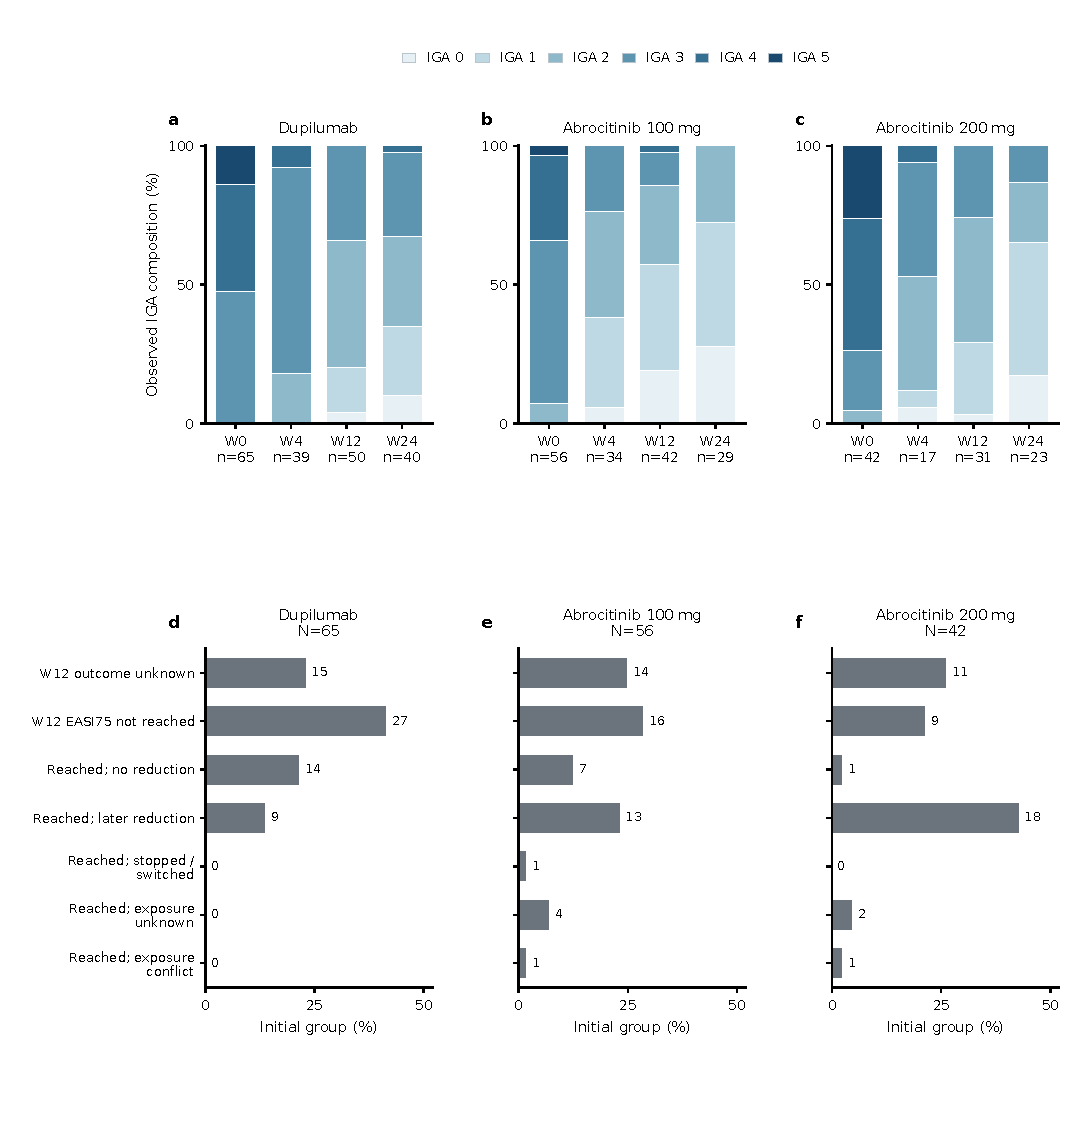
\includegraphics[width=\linewidth,height=.76\textheight,keepaspectratio]{figures/Figure3.pdf}
\caption{\textbf{Molecular response across treatments and the three-marker input panel.} a, Mean paired log$_2$ concentration changes among each marker/treatment-specific fixed set with measurements at W0, W12 and W24. W0 is the zero reference; the two displayed columns per treatment show change to W12 and W24. b, All specified between-treatment contrasts for W0--W12 from HC3-robust linear models, adjusted for starting molecular concentration, W0 EASI, age, BMI, sex and centre; dots denote the declared FDR-adjusted q<0.05. These use all eligible two-visit pairs, a different population from panel a. D, dupilumab; A100/A200, initial abrocitinib dose; pooled A, the observed mixture of the two doses. Both heatmaps use the same signed log$_2$ scale, but panel b is a difference between treatment changes, not a within-group change. Cool blue denotes a negative value, warm coral a positive value; the near-white centre is zero change/difference. Cells marked $\times$ lack an estimate. Panel a prints paired n; $\dagger$ marks fewer than five pairs; these estimates are descriptive. Each estimand has its own labelled colour bar. c--e, W0/W12/W24 paired trajectories and 95\% t confidence intervals for the three frozen model inputs. Their inclusion is based on the existing panel, not selection of significant trajectories. Exact marker-specific counts, intervals, all three windows and the complete comparison families are retained in source tables and supplementary figures.}\label{fig:Figure3}
\end{figure}
\clearpage
\renewcommand{\thefigure}{4}
\begin{figure}[p]
\centering
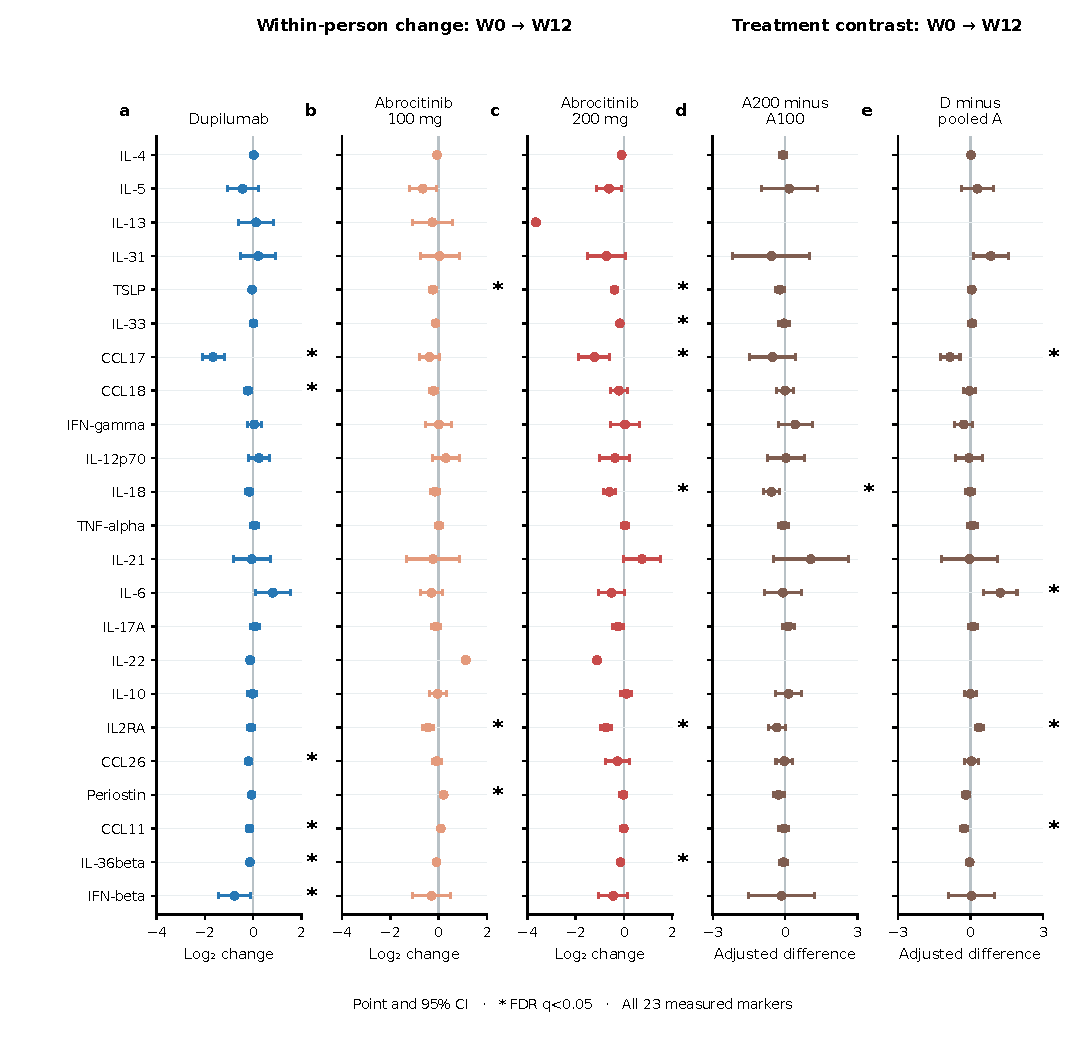
\includegraphics[width=\linewidth,height=.76\textheight,keepaspectratio]{figures/Figure4.pdf}
\caption{\textbf{Individual EASI estimation and its severity boundary.} a--c, Estimated versus observed EASI in the first patient-held-out repetition at W0/W12 and same-cohort temporal application at W24. Each fixed 2$\times$2-EASI-point cell contains all patients whose exact score pair falls within its boundaries. Colour gives patient count on the shared logarithmic count scale; white cells have no observations. All 152/89/75 eligible patients are retained, and identical axes preserve the severity-range comparison. Grey lines denote exact agreement, not a fitted association. d, Cumulative absolute-error proportions, calculated separately in each validation repetition and then averaged. Bands are patient-bootstrap 95\% confidence intervals conditional on saved predictions. All errors enter each proportion; only thresholds from zero to ten points are displayed. The two-point line is a reading reference, not an accepted replacement margin. e, Baseline MAE by observed EASI stratum, with patient-bootstrap 95\% confidence intervals and unique-patient counts. These estimates average the two repetition-specific metrics. W12/W24 have only one/no EASI>21 observation, respectively. W0/W12 use nested patient-level structure and penalty selection; earlier marker selection is not repeated. W24 was previously inspected within the same cohort. These results assess the development procedure, not independent validation of the final formula. Primary overall metrics and numerical controls appear in Table 2; molecular added accuracy has not been established.}\label{fig:Figure4}
\end{figure}
\clearpage
\renewcommand{\thefigure}{5}
\begin{figure}[p]
\centering
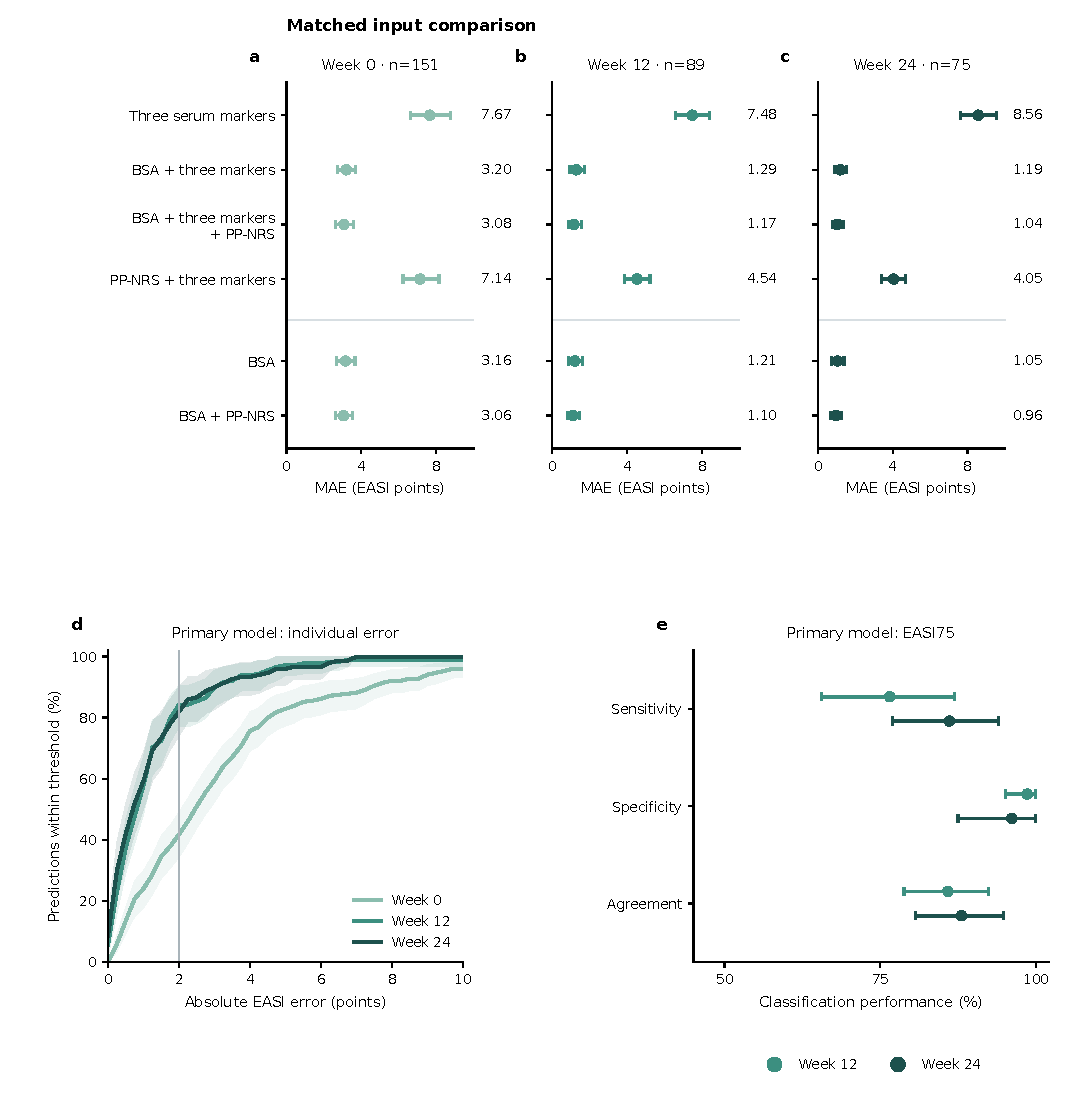
\includegraphics[width=\linewidth,height=.76\textheight,keepaspectratio]{figures/Figure5.pdf}
\caption{\textbf{Within-patient change and EASI75 response classification.} a--c, Estimated versus observed EASI changes in the first patient-held-out repetition. Change is end minus start, so negative values indicate improvement. Fixed 2$\times$2-EASI-point cells count exact paired score changes, using one logarithmic count scale and identical axes across intervals; white cells contain no observations. All 85, 67 and 55 paired patients are retained in their respective windows, which can share patients. Grey diagonal lines denote exact agreement; horizontal and vertical lines mark no change. Primary change MAEs over W0--W12, W0--W24 and W12--W24 are 3.87, 3.47 and 1.49 points, respectively, with intervals in the source tables. These metrics score each of two repetitions before averaging, whereas the count maps illustrate one repetition. d, EASI75 sensitivity, specificity and overall agreement, averaged after classification within each repetition, with patient-bootstrap 95\% confidence intervals conditional on saved predictions. Sensitivity denominators are observed responders (W12 n=49; W24 n=54); specificity denominators are nonresponders (36 and 13). Agreement includes 85 and 67 patients. Observed and estimated response each use their corresponding W0 and follow-up scores; percentage response requires positive observed and estimated W0. W24 is previously inspected same-cohort temporal application, not external validation. Complete EASI50/75/90 classifications and exclusions remain in the supplement. These results assess monitoring agreement, not treatment causality or clinical interchangeability.}\label{fig:Figure5}
\end{figure}
\clearpage
\renewcommand{\thefigure}{S1}
\begin{figure}[p]
\centering
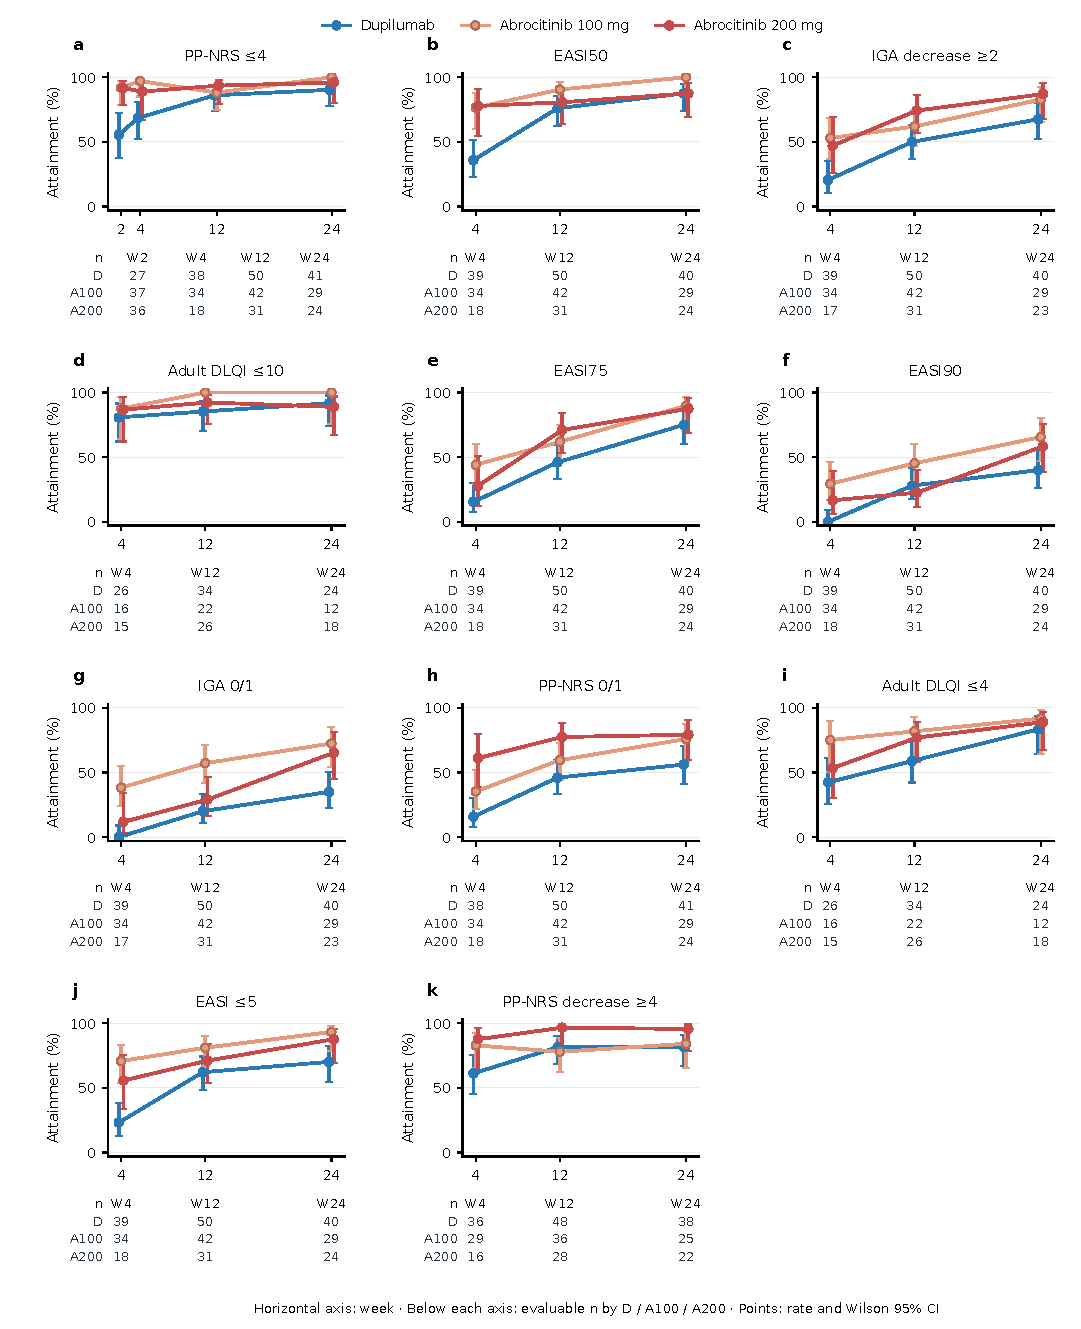
\includegraphics[width=\linewidth,height=.84\textheight,keepaspectratio]{figures/FigureS1.pdf}
\caption{\textbf{Clinical response and absolute-score targets.} Observed proportions with Wilson 95\% confidence intervals, by initial treatment. Count strips give the endpoint-specific evaluable denominator at each visit in D/A100/A200 order. Only PP-NRS $\leq$4 is evaluated at W2. The four-point PP-NRS decrease requires observed baseline PP-NRS $\geq$4 and an observed follow-up value. EASI percentage responses require a positive observed baseline. Adult DLQI requires age $\geq$18. Missing outcomes are unknown, not failures. Connecting lines describe observed visit summaries; the patient set can differ between visits. Initial treatment is retained after regimen changes.}\label{fig:FigureS1}
\end{figure}
\clearpage
\renewcommand{\thefigure}{S2}
\begin{figure}[p]
\centering
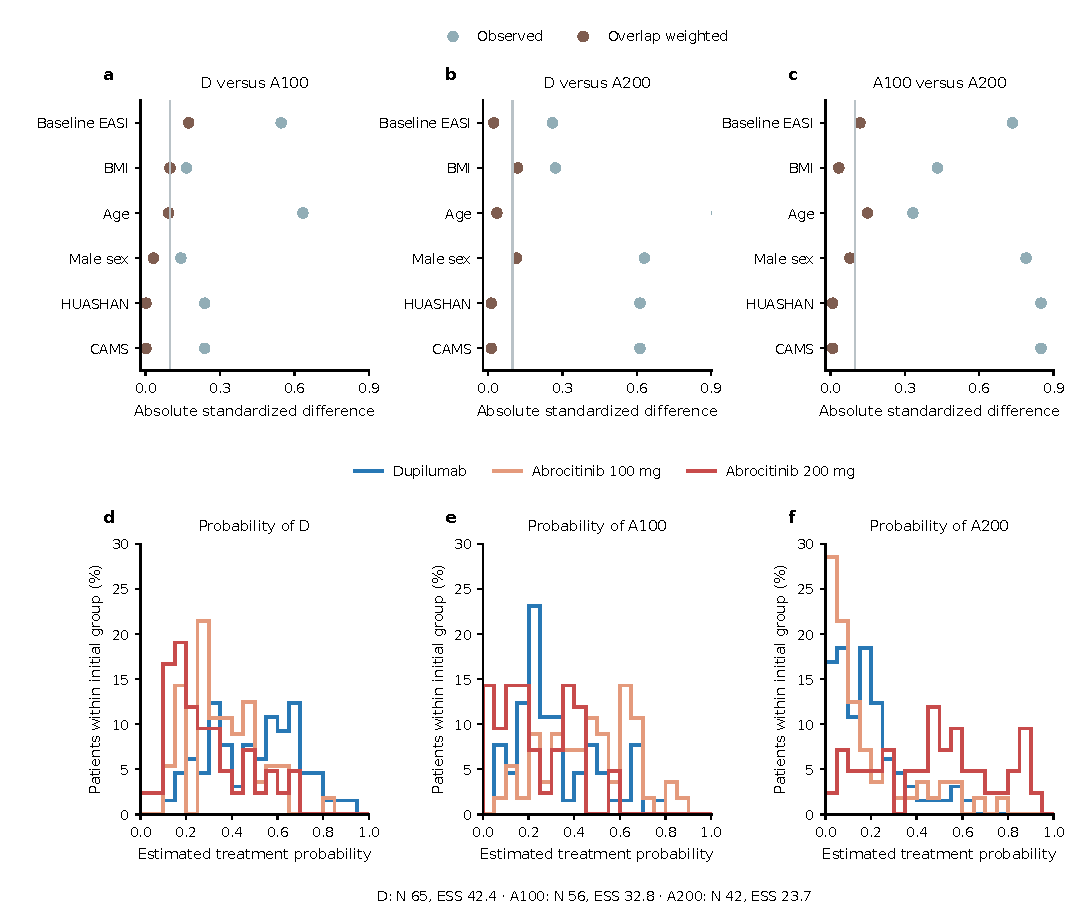
\includegraphics[width=\linewidth,height=.84\textheight,keepaspectratio]{figures/FigureS2.pdf}
\caption{\textbf{Observed and baseline-adjusted EASI, PP-NRS, Adult DLQI.} Each row is one outcome. Left, overall available-case mean and 95\% t confidence interval, exactly combined from group moments. Middle, initial-treatment-specific median and interquartile range. Right, overlap-weighted adjusted trajectories and patient-cluster robust 95\% confidence intervals, controlling baseline outcome, age, sex, BMI and centre. Visit composition may change. Only investigator-specified visits are shown; no causal current-dose effect is claimed. Exact sample sizes and contrasts accompany the source tables.}\label{fig:FigureS2}
\end{figure}
\clearpage
\renewcommand{\thefigure}{S3}
\begin{figure}[p]
\centering
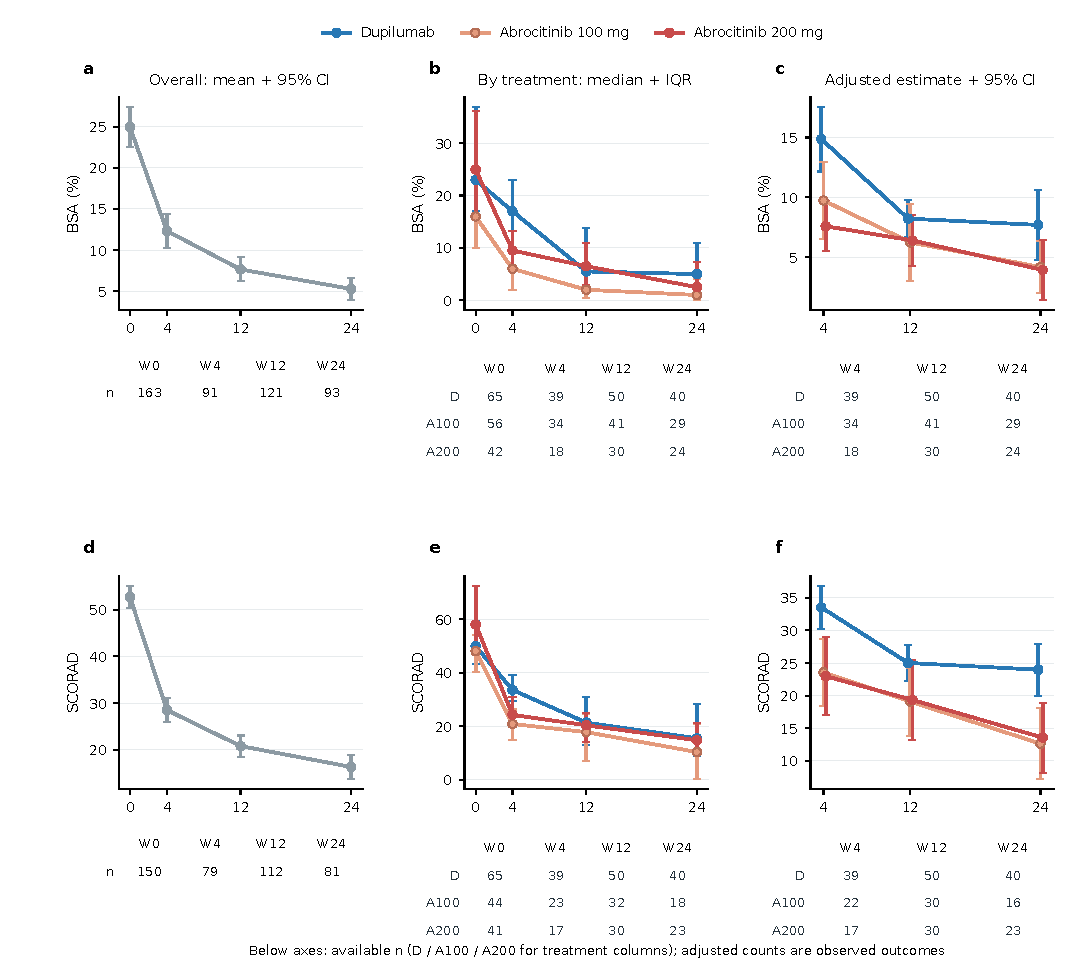
\includegraphics[width=\linewidth,height=.84\textheight,keepaspectratio]{figures/FigureS3.pdf}
\caption{\textbf{Observed and baseline-adjusted BSA (\%), SCORAD.} Each row is one outcome. Left, overall available-case mean and 95\% t confidence interval, exactly combined from group moments. Middle, initial-treatment-specific median and interquartile range. Right, overlap-weighted adjusted trajectories and patient-cluster robust 95\% confidence intervals, controlling baseline outcome, age, sex, BMI and centre. Visit composition may change. Only investigator-specified visits are shown; no causal current-dose effect is claimed. Exact sample sizes and contrasts accompany the source tables.}\label{fig:FigureS3}
\end{figure}
\clearpage
\renewcommand{\thefigure}{S4}
\begin{figure}[p]
\centering
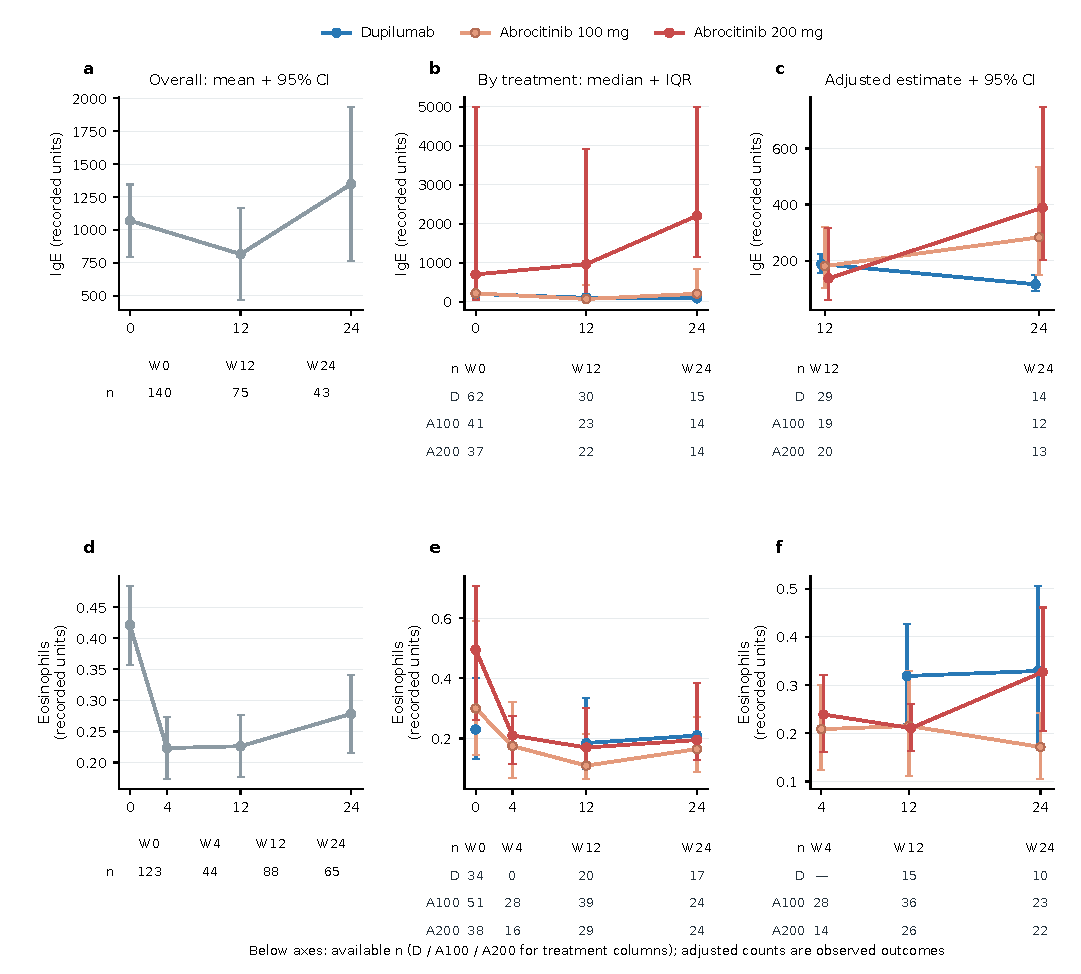
\includegraphics[width=\linewidth,height=.84\textheight,keepaspectratio]{figures/FigureS4.pdf}
\caption{\textbf{Observed and baseline-adjusted IgE (recorded units), Eosinophils (recorded units).} Each row is one outcome. Left, overall available-case mean and 95\% t confidence interval, exactly combined from group moments. Middle, initial-treatment-specific median and interquartile range. Right, overlap-weighted adjusted trajectories and patient-cluster robust 95\% confidence intervals, controlling baseline outcome, age, sex, BMI and centre. IgE/eosinophils use log(1+x) models and back-transformation; these adjusted estimates are not arithmetic means. Visit composition may change. Only investigator-specified visits are shown; no causal current-dose effect is claimed. Exact sample sizes and contrasts accompany the source tables.}\label{fig:FigureS4}
\end{figure}
\clearpage
\renewcommand{\thefigure}{S5}
\begin{figure}[p]
\centering
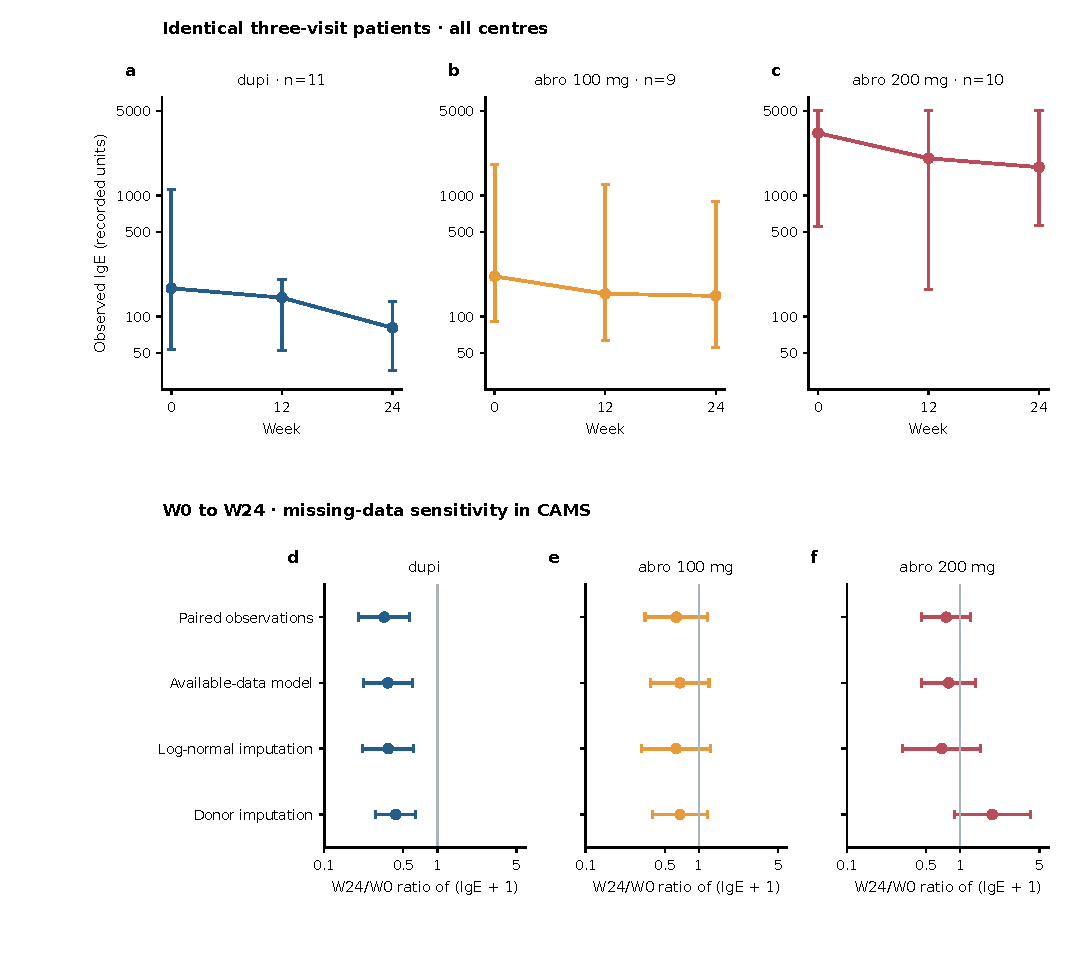
\includegraphics[width=\linewidth,height=.84\textheight,keepaspectratio]{figures/FigureS5.pdf}
\caption{\textbf{All molecular changes within W0 $\rightarrow$ W12.} Mean within-patient log$_2$ concentration changes and 95\% t confidence intervals. Negative values mean a decline: $-$1 equals a geometric paired ratio of 0.5. Each marker/treatment uses its available pairs, shown as [n]; sets may differ between windows. Points with fewer than five pairs are descriptive and have no inferential interval; rows without an estimable mean are marked NE (not estimable) in the outside status column. Stars indicate BH q<0.05 across the full 207 marker-by-treatment-by-window family. All 23 measured markers are included.}\label{fig:FigureS5}
\end{figure}
\clearpage
\renewcommand{\thefigure}{S6}
\begin{figure}[p]
\centering
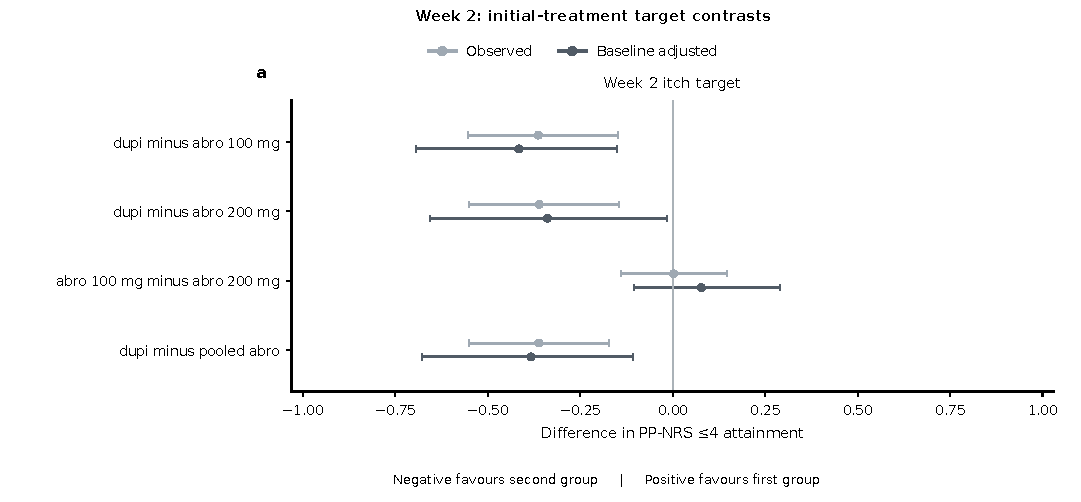
\includegraphics[width=\linewidth,height=.84\textheight,keepaspectratio]{figures/FigureS6.pdf}
\caption{\textbf{All molecular changes within W12 $\rightarrow$ W24.} Mean within-patient log$_2$ concentration changes and 95\% t confidence intervals. Negative values mean a decline: $-$1 equals a geometric paired ratio of 0.5. Each marker/treatment uses its available pairs, shown as [n]; sets may differ between windows. Points with fewer than five pairs are descriptive and have no inferential interval; rows without an estimable mean are marked NE (not estimable) in the outside status column. Stars indicate BH q<0.05 across the full 207 marker-by-treatment-by-window family. All 23 measured markers are included.}\label{fig:FigureS6}
\end{figure}
\clearpage
\renewcommand{\thefigure}{S7}
\begin{figure}[p]
\centering
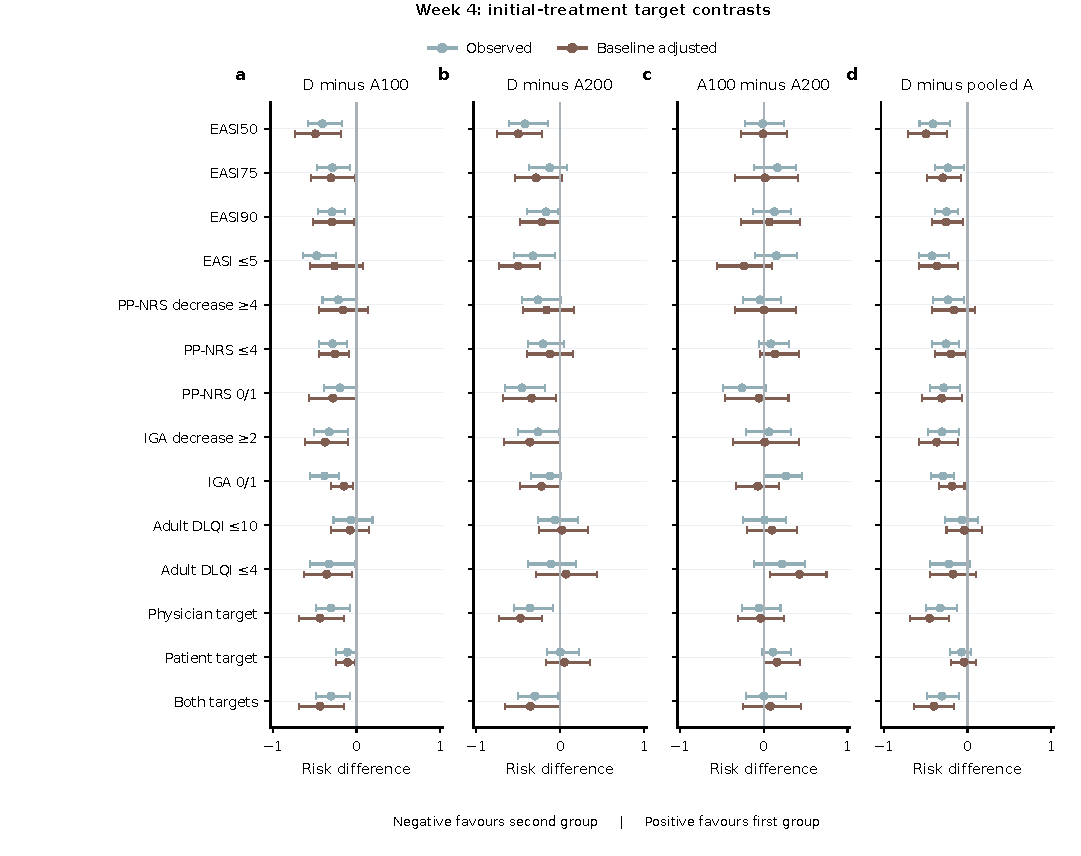
\includegraphics[width=\linewidth,height=.84\textheight,keepaspectratio]{figures/FigureS7.pdf}
\caption{\textbf{All molecular changes within W0 $\rightarrow$ W24.} Mean within-patient log$_2$ concentration changes and 95\% t confidence intervals. Negative values mean a decline: $-$1 equals a geometric paired ratio of 0.5. Each marker/treatment uses its available pairs, shown as [n]; sets may differ between windows. Points with fewer than five pairs are descriptive and have no inferential interval; rows without an estimable mean are marked NE (not estimable) in the outside status column. Stars indicate BH q<0.05 across the full 207 marker-by-treatment-by-window family. All 23 measured markers are included.}\label{fig:FigureS7}
\end{figure}
\clearpage
\renewcommand{\thefigure}{S8}
\begin{figure}[p]
\centering
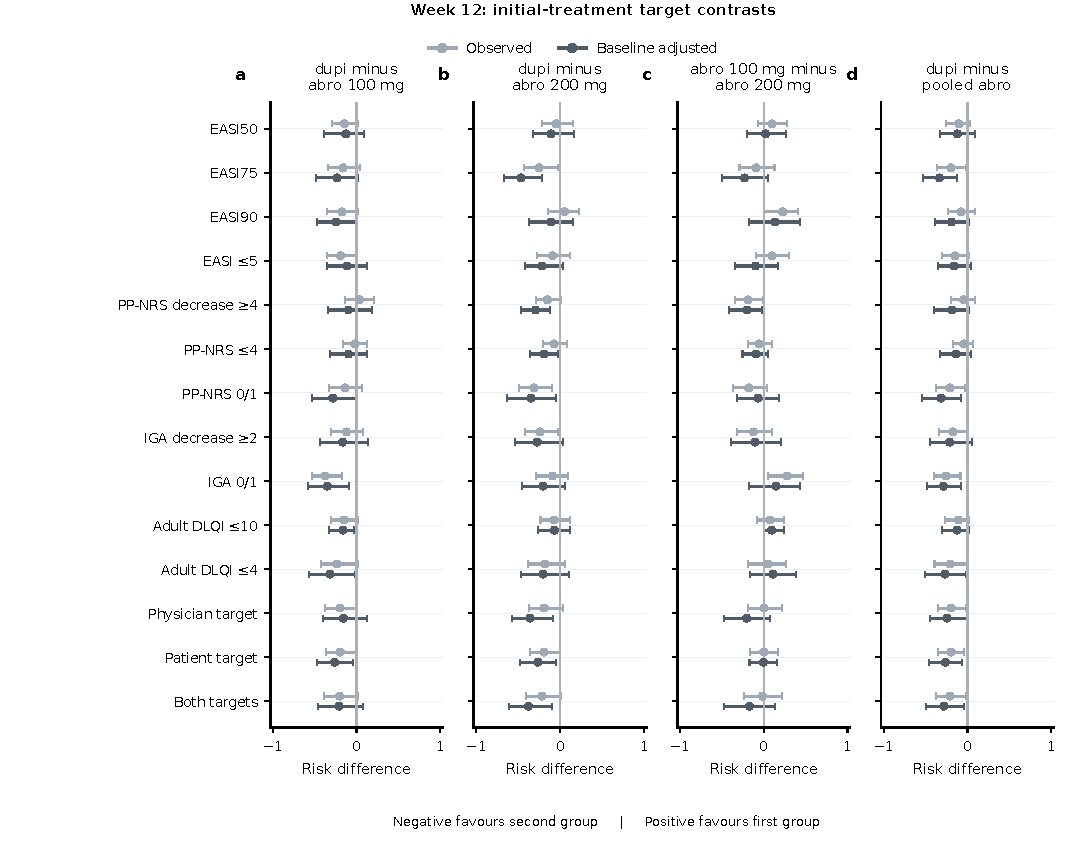
\includegraphics[width=\linewidth,height=.84\textheight,keepaspectratio]{figures/FigureS8.pdf}
\caption{\textbf{Adjusted treatment contrasts in molecular change: W0 $\rightarrow$ W12.} Baseline-adjusted contrasts with HC3 95\% confidence intervals. All 23 markers and four contrasts are shown. D denotes dupilumab and A100/A200 initial abrocitinib doses. Negative means the first treatment has a smaller, more negative change; it is not a negative concentration. Models control starting log$_2$ concentration, baseline total EASI, age, sex, BMI and centre; source tables provide exact n, exclusions, BH q values, centre and batch sensitivities. Pooled abrocitinib retains the observed initial-dose mixture. These are observational initial-treatment contrasts, not randomized current-dose effects.}\label{fig:FigureS8}
\end{figure}
\clearpage
\renewcommand{\thefigure}{S9}
\begin{figure}[p]
\centering
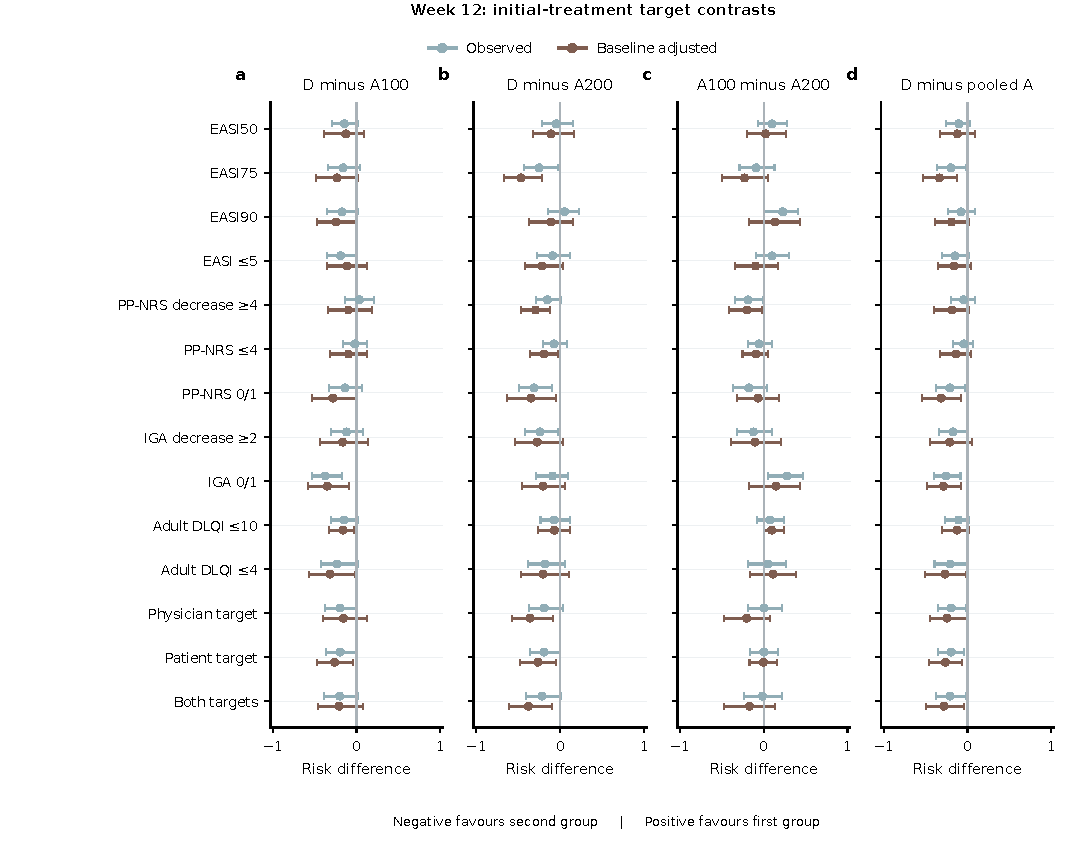
\includegraphics[width=\linewidth,height=.84\textheight,keepaspectratio]{figures/FigureS9.pdf}
\caption{\textbf{Adjusted treatment contrasts in molecular change: W12 $\rightarrow$ W24.} Baseline-adjusted contrasts with HC3 95\% confidence intervals. All 23 markers and four contrasts are shown. D denotes dupilumab and A100/A200 initial abrocitinib doses. Negative means the first treatment has a smaller, more negative change; it is not a negative concentration. Models control starting log$_2$ concentration, baseline total EASI, age, sex, BMI and centre; source tables provide exact n, exclusions, BH q values, centre and batch sensitivities. Pooled abrocitinib retains the observed initial-dose mixture. These are observational initial-treatment contrasts, not randomized current-dose effects.}\label{fig:FigureS9}
\end{figure}
\clearpage
\renewcommand{\thefigure}{S10}
\begin{figure}[p]
\centering
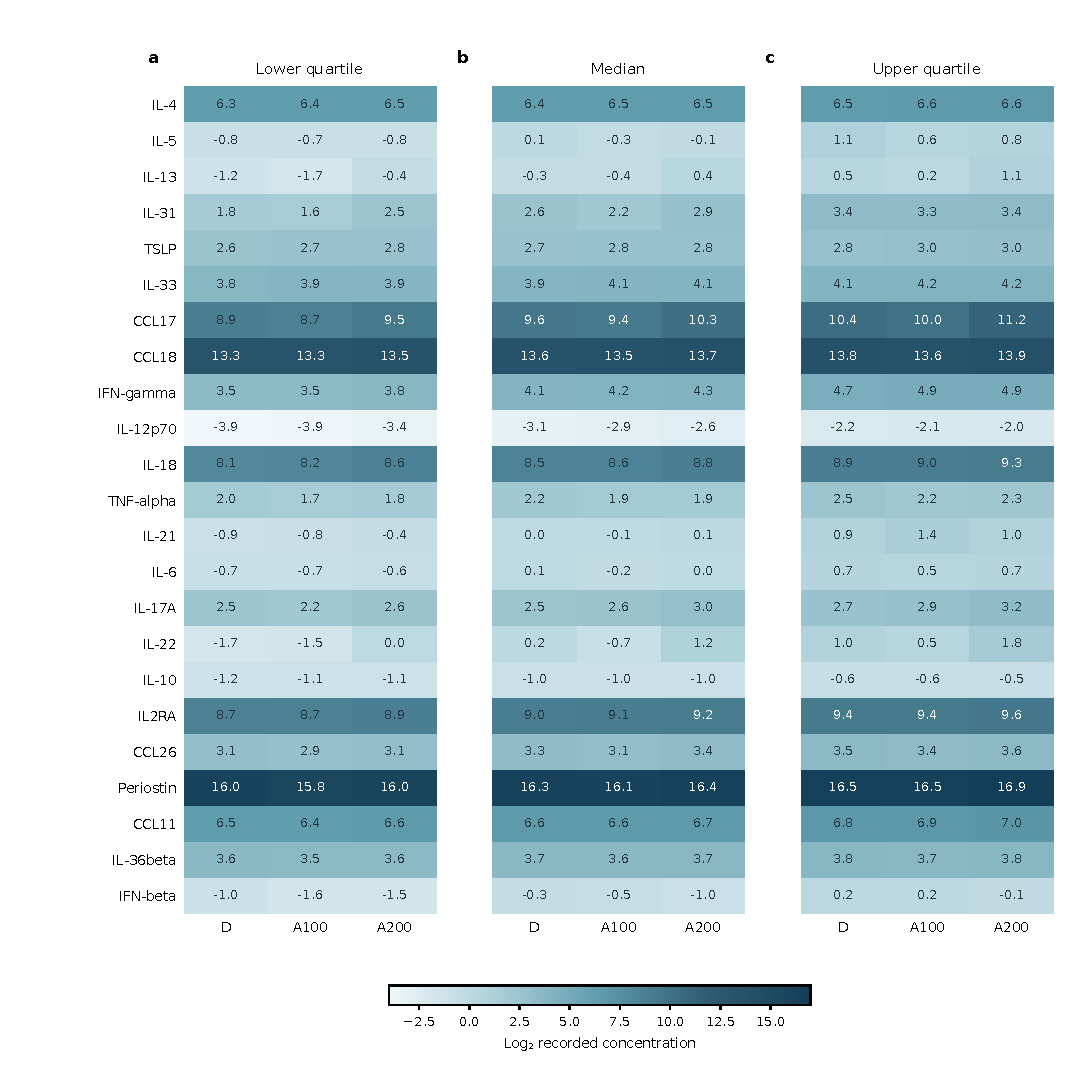
\includegraphics[width=\linewidth,height=.84\textheight,keepaspectratio]{figures/FigureS10.pdf}
\caption{\textbf{Adjusted treatment contrasts in molecular change: W0 $\rightarrow$ W24.} Baseline-adjusted contrasts with HC3 95\% confidence intervals. All 23 markers and four contrasts are shown. D denotes dupilumab and A100/A200 initial abrocitinib doses. Negative means the first treatment has a smaller, more negative change; it is not a negative concentration. Models control starting log$_2$ concentration, baseline total EASI, age, sex, BMI and centre; source tables provide exact n, exclusions, BH q values, centre and batch sensitivities. Pooled abrocitinib retains the observed initial-dose mixture. These are observational initial-treatment contrasts, not randomized current-dose effects.}\label{fig:FigureS10}
\end{figure}
\clearpage
\renewcommand{\thefigure}{S11}
\begin{figure}[p]
\centering
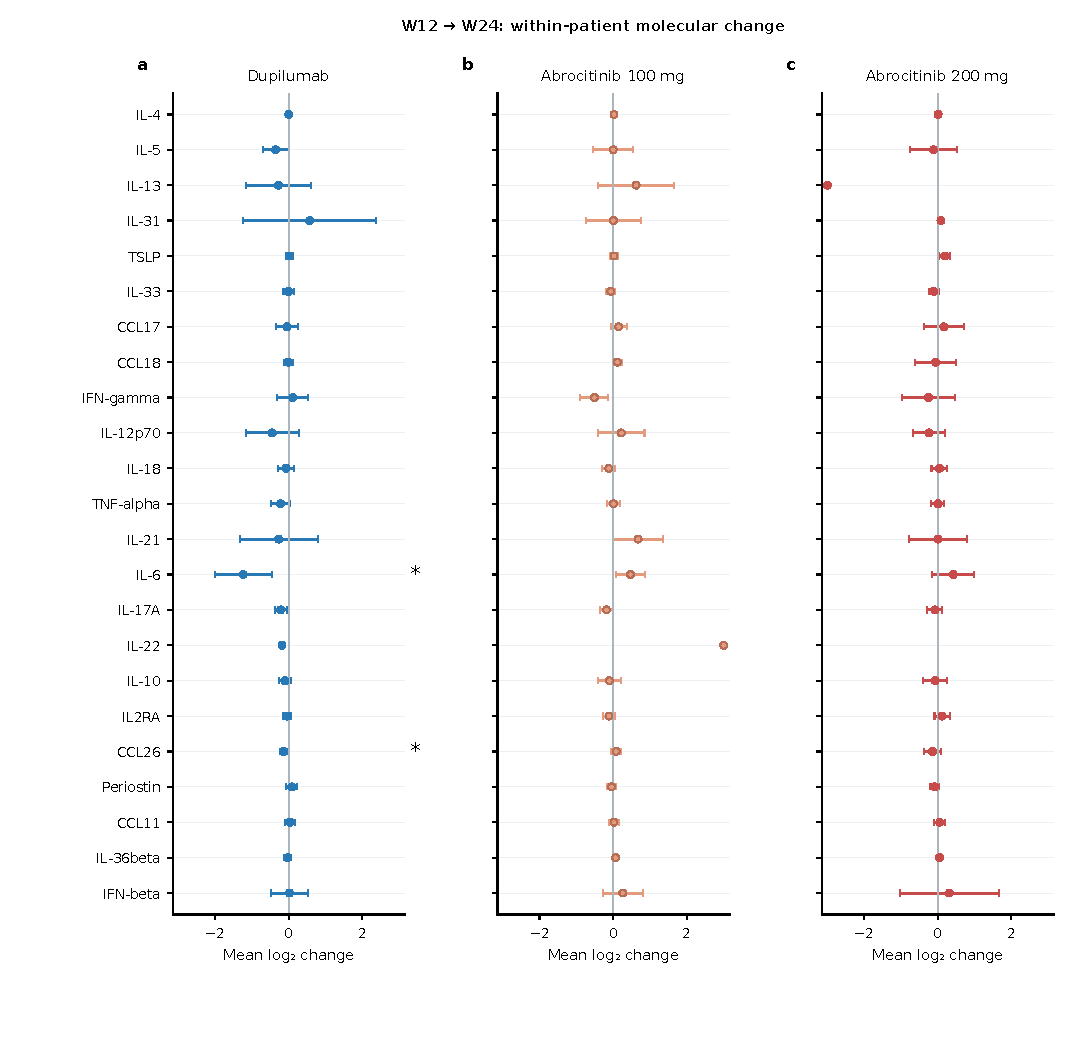
\includegraphics[width=\linewidth,height=.84\textheight,keepaspectratio]{figures/FigureS11.pdf}
\caption{\textbf{Clinical--molecular change associations: W0 $\rightarrow$ W12.} Colour is Spearman correlation between paired clinical change and paired log$_2$ molecular change, both later minus earlier. Cell numbers show complete-pair patient counts and stars BH q<0.05. Positive correlations indicate changes in the same direction; negative correlations indicate opposite changes. Cells marked $\times$ have no estimable correlation; printed n distinguishes no pairs from an unestimable coefficient among available pairs. Daggers flag descriptive small cells with n<5. Adult DLQI requires age $\geq$18. Correlation does not establish numerical interchangeability or causal effects. All coefficients, bootstrap confidence intervals and multiplicity-adjusted tests remain in source data.}\label{fig:FigureS11}
\end{figure}
\clearpage
\renewcommand{\thefigure}{S12}
\begin{figure}[p]
\centering
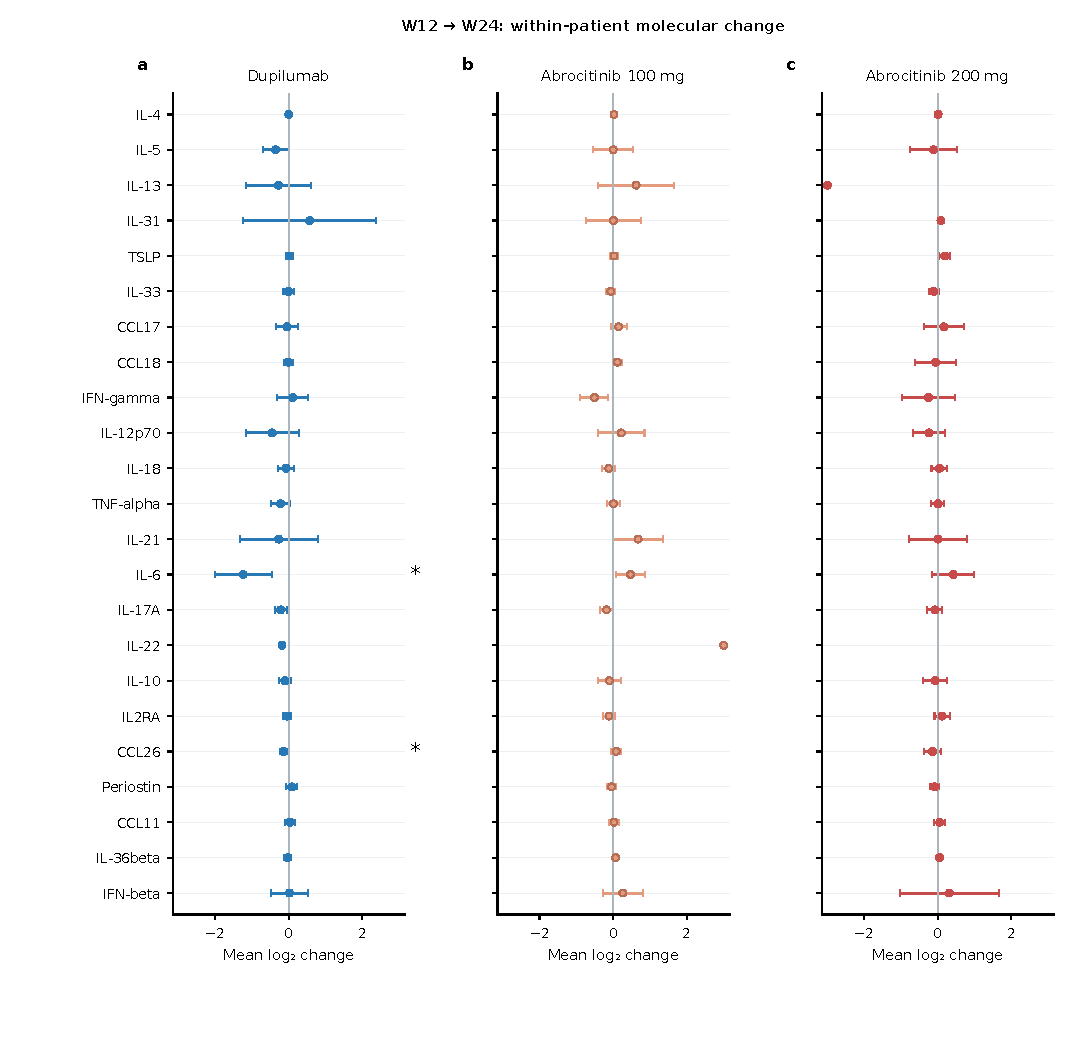
\includegraphics[width=\linewidth,height=.84\textheight,keepaspectratio]{figures/FigureS12.pdf}
\caption{\textbf{Clinical--molecular change associations: W12 $\rightarrow$ W24.} Colour is Spearman correlation between paired clinical change and paired log$_2$ molecular change, both later minus earlier. Cell numbers show complete-pair patient counts and stars BH q<0.05. Positive correlations indicate changes in the same direction; negative correlations indicate opposite changes. Cells marked $\times$ have no estimable correlation; printed n distinguishes no pairs from an unestimable coefficient among available pairs. Daggers flag descriptive small cells with n<5. Adult DLQI requires age $\geq$18. Correlation does not establish numerical interchangeability or causal effects. All coefficients, bootstrap confidence intervals and multiplicity-adjusted tests remain in source data.}\label{fig:FigureS12}
\end{figure}
\clearpage
\renewcommand{\thefigure}{S13}
\begin{figure}[p]
\centering
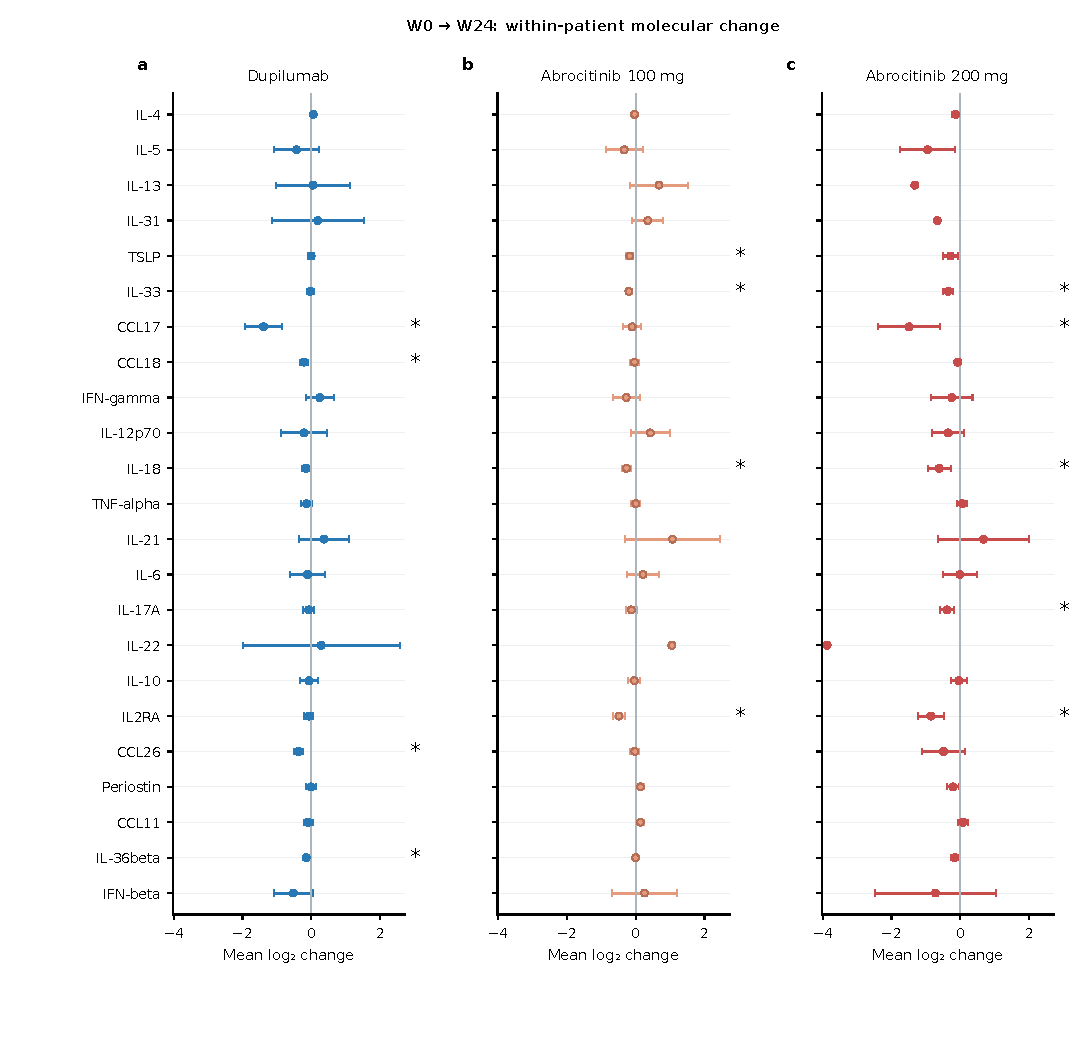
\includegraphics[width=\linewidth,height=.84\textheight,keepaspectratio]{figures/FigureS13.pdf}
\caption{\textbf{Clinical--molecular change associations: W0 $\rightarrow$ W24.} Colour is Spearman correlation between paired clinical change and paired log$_2$ molecular change, both later minus earlier. Cell numbers show complete-pair patient counts and stars BH q<0.05. Positive correlations indicate changes in the same direction; negative correlations indicate opposite changes. Cells marked $\times$ have no estimable correlation; printed n distinguishes no pairs from an unestimable coefficient among available pairs. Daggers flag descriptive small cells with n<5. Adult DLQI requires age $\geq$18. Correlation does not establish numerical interchangeability or causal effects. All coefficients, bootstrap confidence intervals and multiplicity-adjusted tests remain in source data.}\label{fig:FigureS13}
\end{figure}
\clearpage
\renewcommand{\thefigure}{S14}
\begin{figure}[p]
\centering
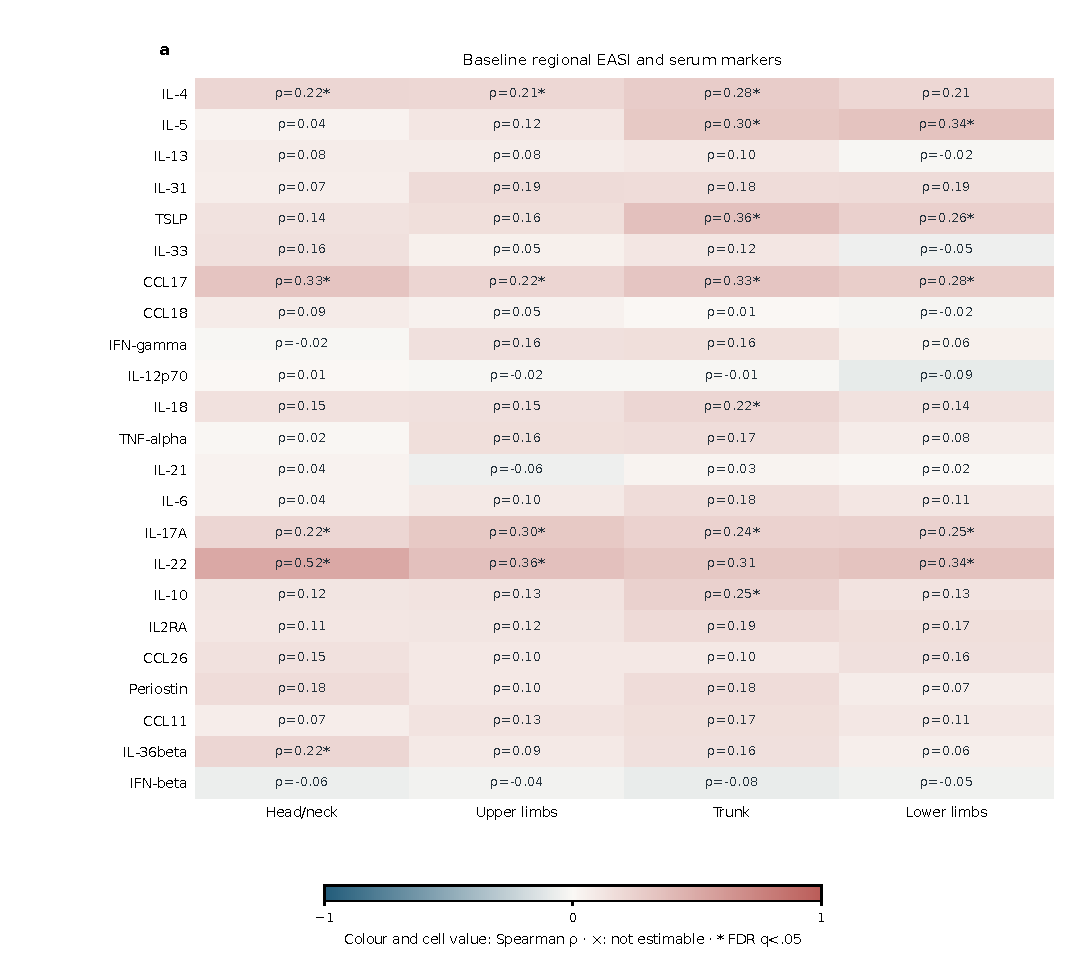
\includegraphics[width=\linewidth,height=.84\textheight,keepaspectratio]{figures/FigureS14.pdf}
\caption{\textbf{Baseline molecular associations with four skin regions.} Observed baseline Spearman correlations pooled across initial-treatment groups, using source-consistent regional EASI and matched serum measurements. Values are printed in cells; stars indicate BH q<0.05. Regional records must be complete, within theoretical bounds and sum to total EASI within 0.01. Counts and bootstrap confidence intervals are in the source table. Serum association alone does not establish site-specific pathogenesis.}\label{fig:FigureS14}
\end{figure}
\clearpage
\renewcommand{\thefigure}{S15}
\begin{figure}[p]
\centering
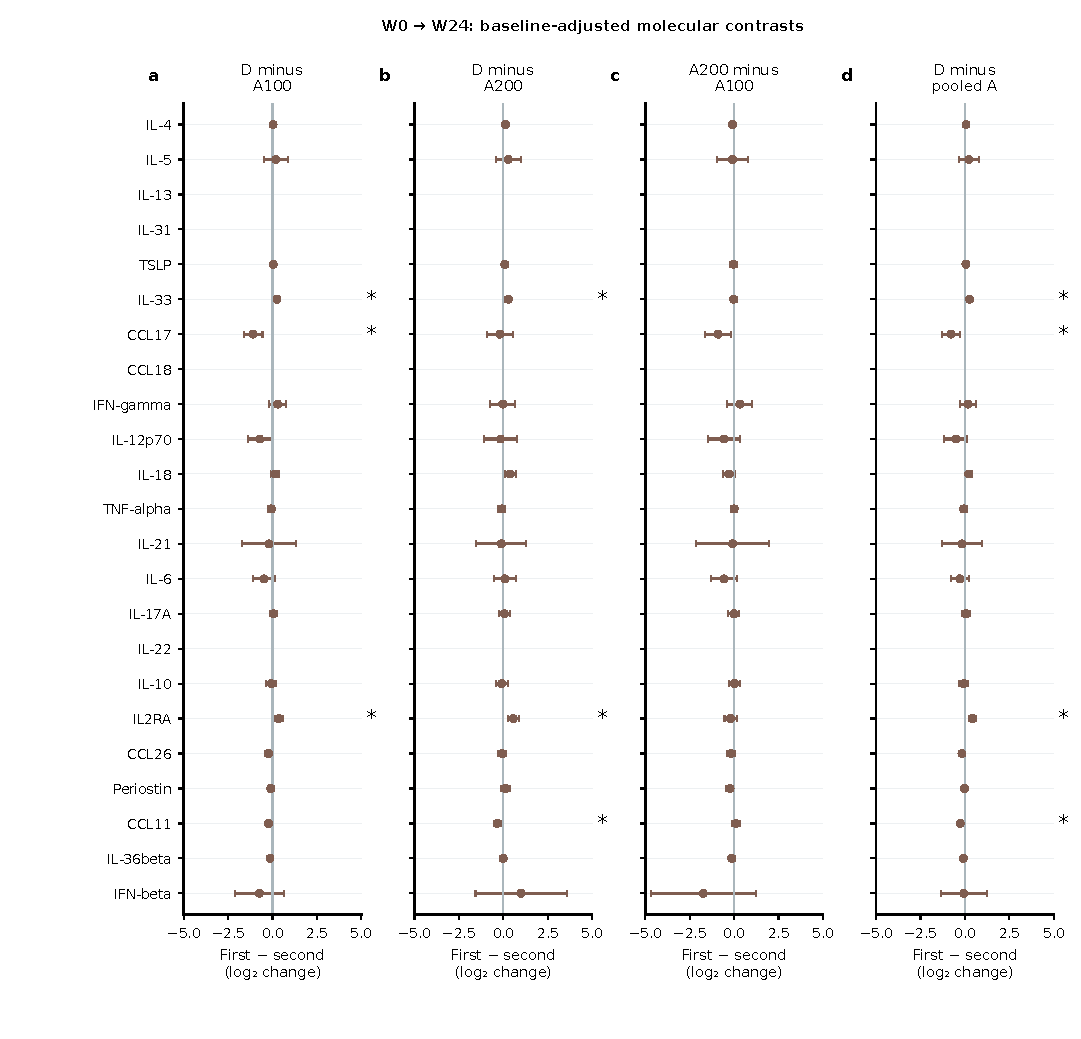
\includegraphics[width=\linewidth,height=.84\textheight,keepaspectratio]{figures/FigureS15.pdf}
\caption{\textbf{Recorded IGA composition at four visits.} Each bar is the recorded IGA composition among evaluable patients, whose total n is printed below the bar. The ordered blue scale encodes recorded grade 0--5, not treatment; borders distinguish grade 0 from the background. Labels in segments occupying at least 10\% show grade and exact patient count; all grade counts remain in source data. Grade 5 remains as recorded because instrument identity is unresolved; no conversion to a standard 0--4 scale was made. EASI90 is shown with the other clinical targets in Figure S1.}\label{fig:FigureS15}
\end{figure}
\clearpage
\renewcommand{\thefigure}{S16}
\begin{figure}[p]
\centering
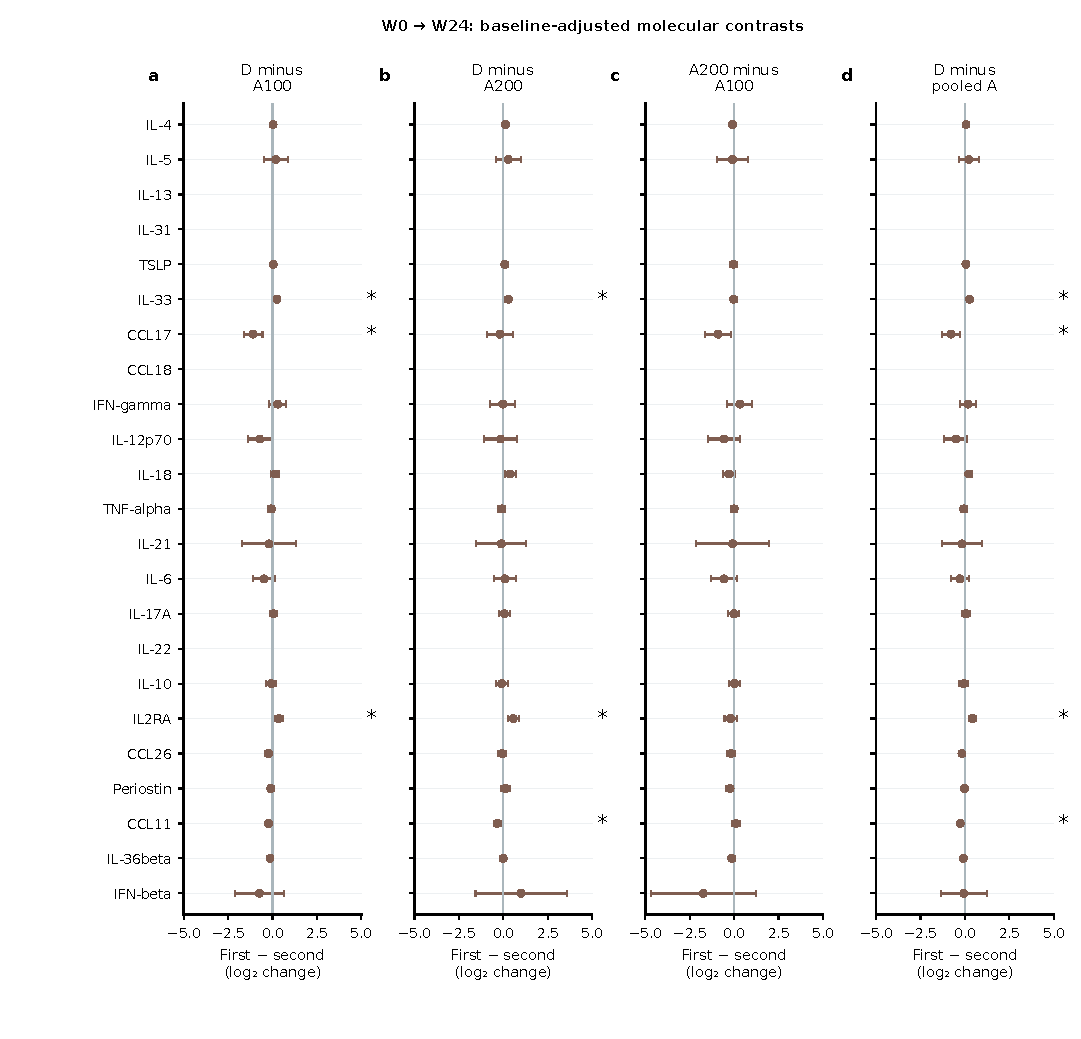
\includegraphics[width=\linewidth,height=.84\textheight,keepaspectratio]{figures/FigureS16.pdf}
\caption{\textbf{EASI trajectories before and after the W12 treatment decision.} Each panel is one recorded pathway: W12 EASI75 not reached, reached without recorded reduction, or reached followed by reduction. All trajectories retain the same patients observed at W0/W12/W24; treatment is encoded by colour with solid lines and circle markers. Median and patient-bootstrap 95\% confidence intervals are shown. Panel counts are ordered D/A100/A200; the zero-size A200 group in the no-reduction panel has no trajectory. Paths depend on later information and are descriptive, not randomized treatment strategies. Other paths, including unknown exposure, stopping and switching, remain in the source tables.}\label{fig:FigureS16}
\end{figure}
\clearpage
\renewcommand{\thefigure}{S17}
\begin{figure}[p]
\centering
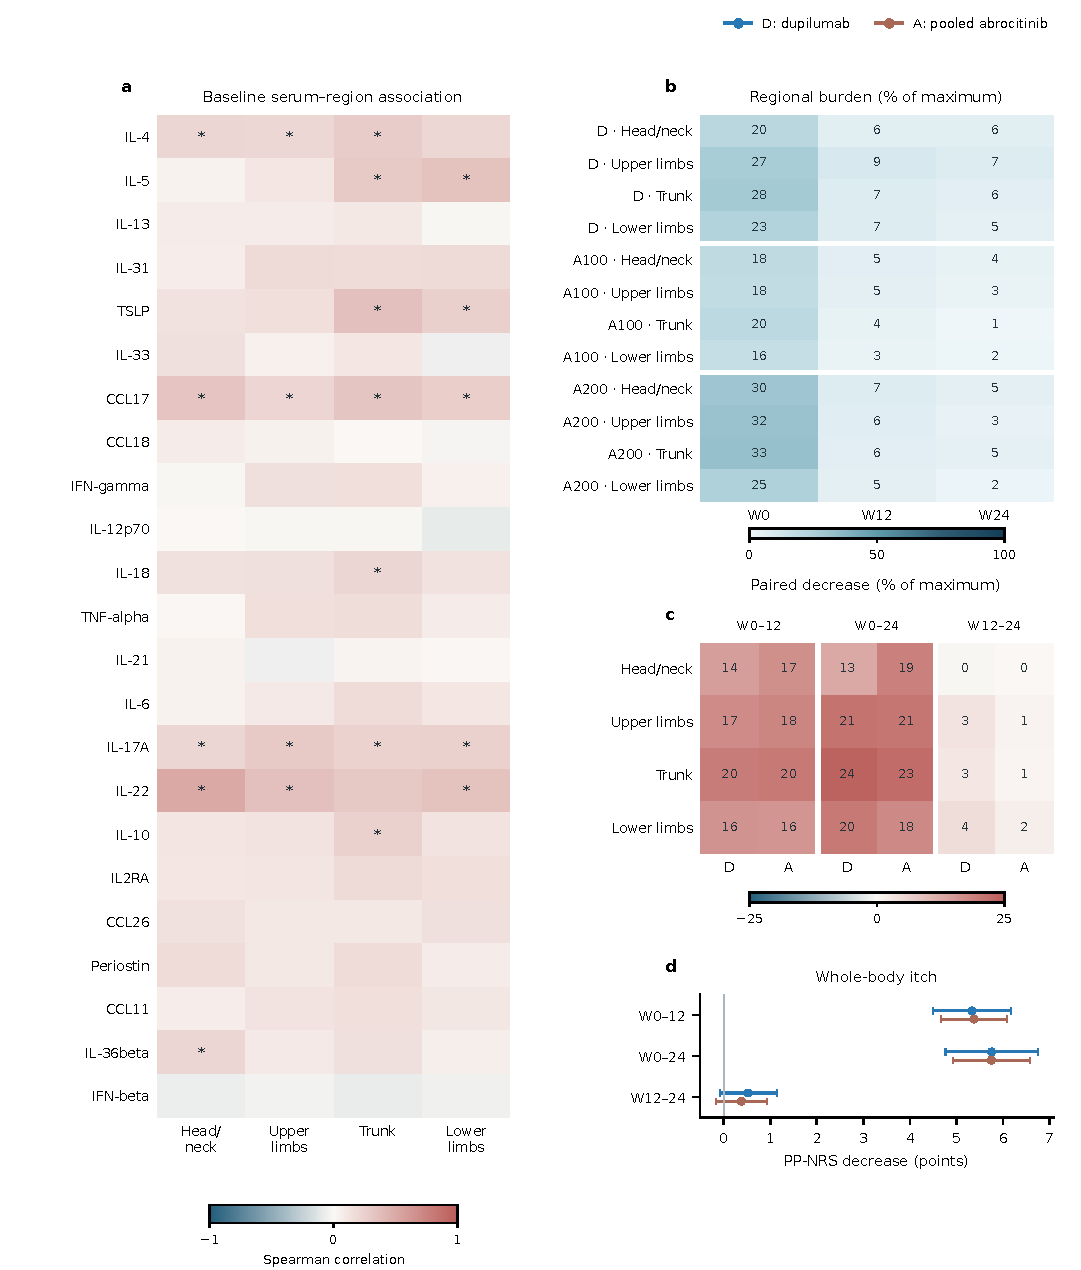
\includegraphics[width=\linewidth,height=.84\textheight,keepaspectratio]{figures/FigureS17.pdf}
\caption{\textbf{W24 EASI75 status in future-defined recorded pathways.} Each row shows the observed W24 EASI75 proportion and Wilson 95\% confidence interval among evaluable patients. The table states complete pathway size N, attained/evaluable k/eval and the count missing a W24 score. All recorded paths are retained, including zero-size rows, which explicitly show N=0 and Not estimable. An evaluable denominator of zero is not a zero response rate. W12 target status and later recorded treatment define these pathways; they are descriptive future-defined groups, not randomized strategies or causal tapering effects. Missing outcomes are unknown, not failures. Missing-outcome bounds remain in source data.}\label{fig:FigureS17}
\end{figure}
\clearpage
\renewcommand{\thefigure}{S18}
\begin{figure}[p]
\centering
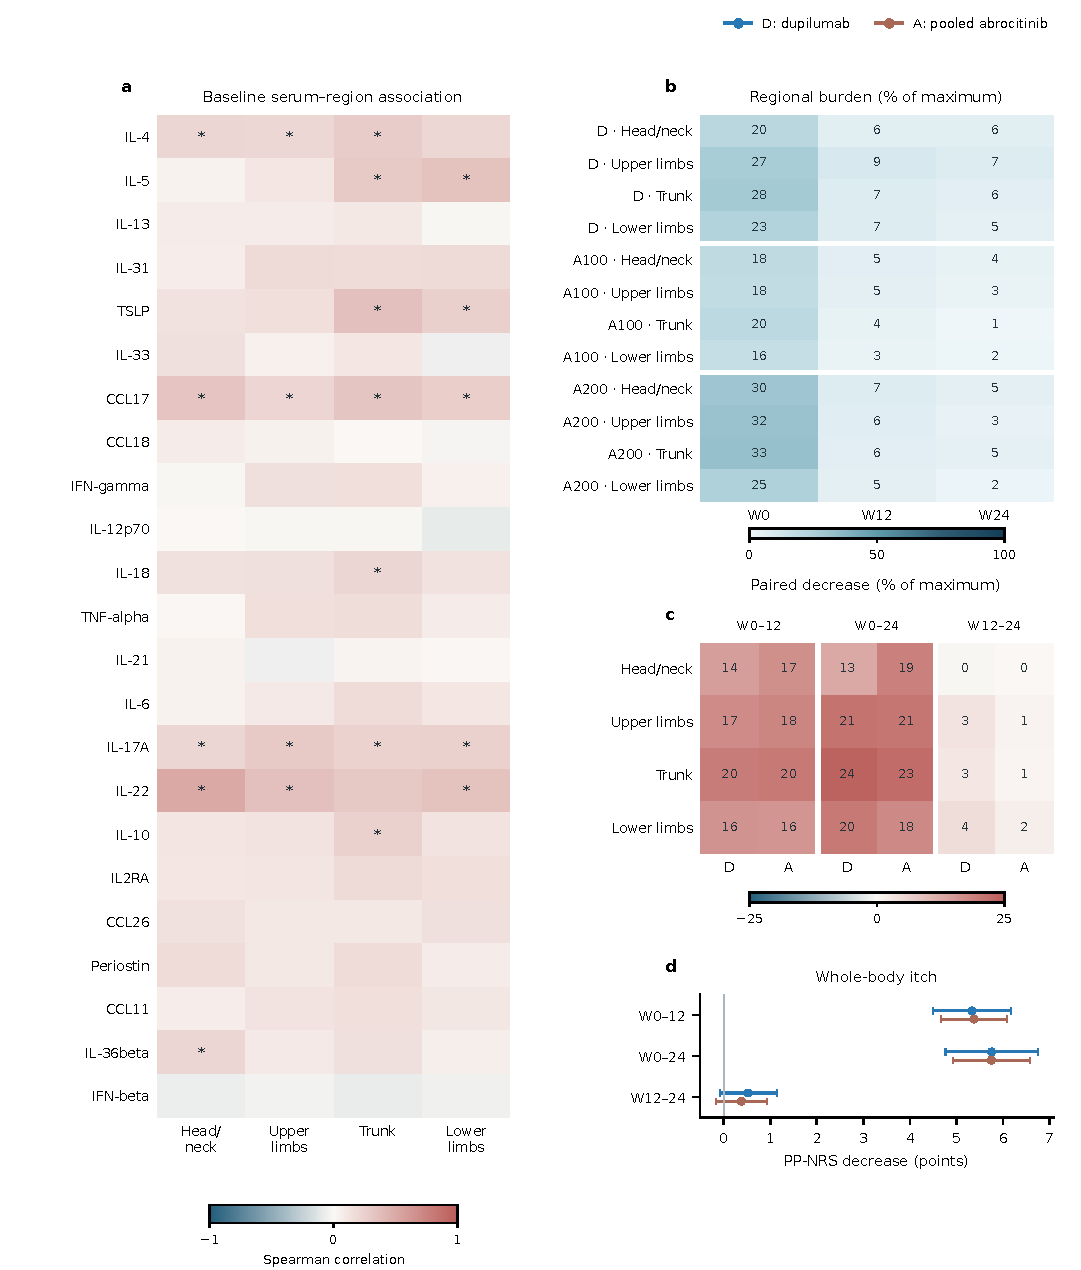
\includegraphics[width=\linewidth,height=.84\textheight,keepaspectratio]{figures/FigureS18.pdf}
\caption{\textbf{Baseline concentration distributions for the full measured panel.} Baseline medians and interquartile ranges of log$_2$ recorded concentrations, with available patient counts [n]. Treatment colours are fixed across the manuscript. Compare treatment groups within each marker; absolute values across different analytes do not represent comparable biological activity. All 23 markers are retained, including sparse or censored assays. Censoring and repeated values are separately audited.}\label{fig:FigureS18}
\end{figure}
\clearpage
\renewcommand{\thefigure}{S19}
\begin{figure}[p]
\centering
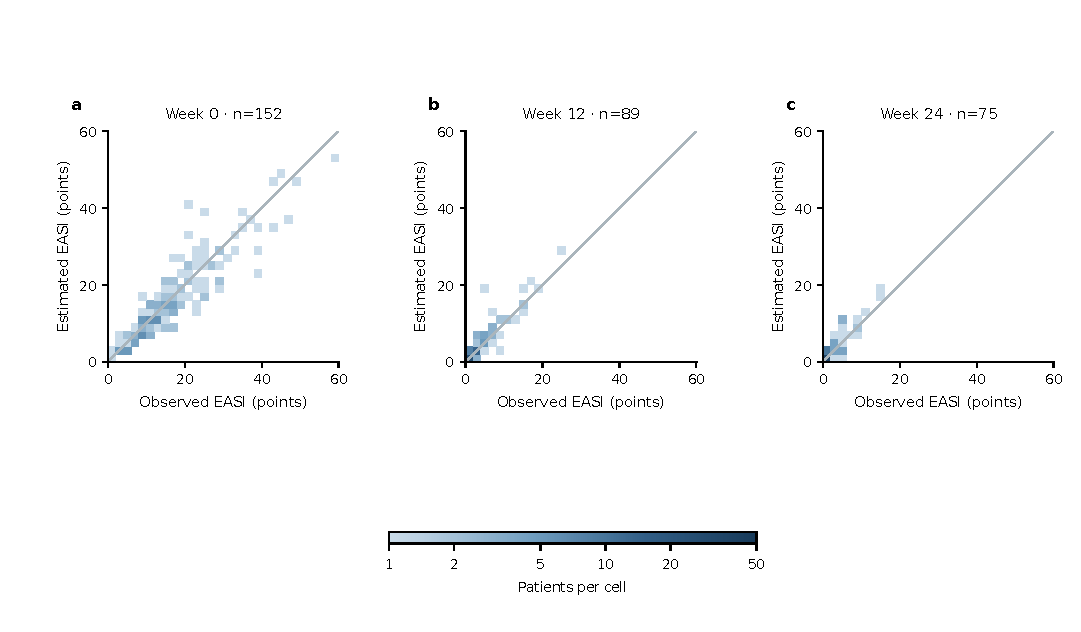
\includegraphics[width=\linewidth,height=.84\textheight,keepaspectratio]{figures/FigureS19.pdf}
\caption{\textbf{Molecular W0/W12/W24 changes in identical patient sets.} Within each marker and initial treatment, all three colours use the same patients observed at W0/W12/W24. Fixed triplet counts are shown as [n]. W0 equals zero by definition; W12/W24 are mean within-patient log$_2$ changes from W0 with 95\% t confidence intervals when n$\geq$5. Sets with n<5 are descriptive and have no inferential interval. Negative values indicate lower concentration, not absence of the analyte. This includes every measured marker and its uncertainty, complementing the overview heatmap.}\label{fig:FigureS19}
\end{figure}
\clearpage
\renewcommand{\thefigure}{S20}
\begin{figure}[p]
\centering
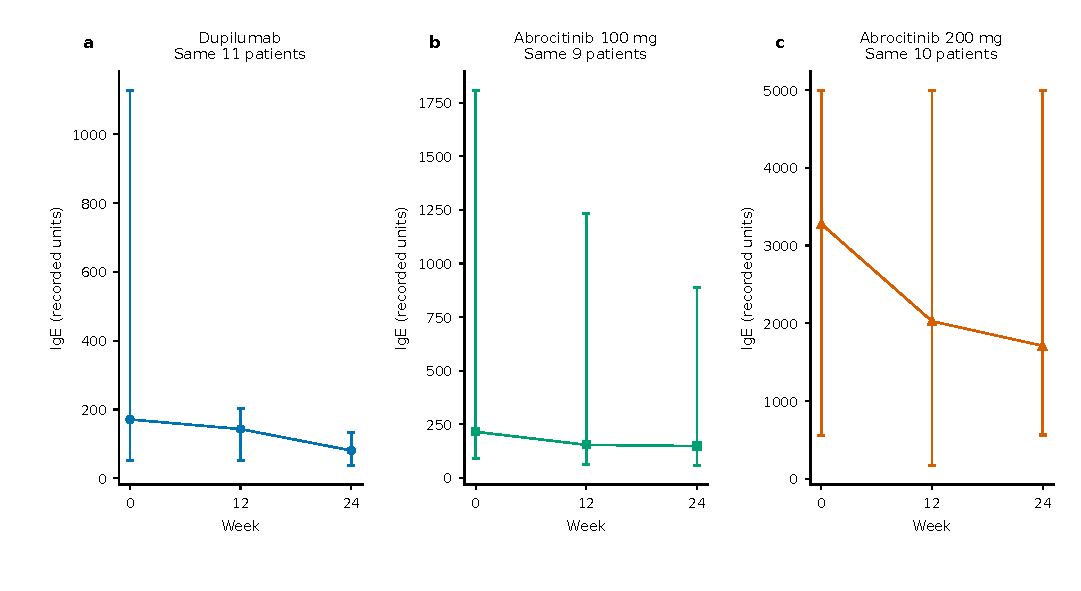
\includegraphics[width=\linewidth,height=.84\textheight,keepaspectratio]{figures/FigureS20.pdf}
\caption{\textbf{IgE with the same patients retained at all three visits.} Medians and patient-bootstrap 95\% confidence intervals in fixed complete W0/W12/W24 sets. Each treatment panel retains identical patients at all three visits. Vertical scales differ across treatment panels so that within-group trajectories remain visible; compare absolute values using the tick labels. These denominators differ from cross-sectional and W0--W24-only paired sets. This figure tests whether changing sample composition may explain an apparent visit-level rise; it does not establish a causal drug effect.}\label{fig:FigureS20}
\end{figure}
\clearpage
\renewcommand{\thefigure}{S21}
\begin{figure}[p]
\centering
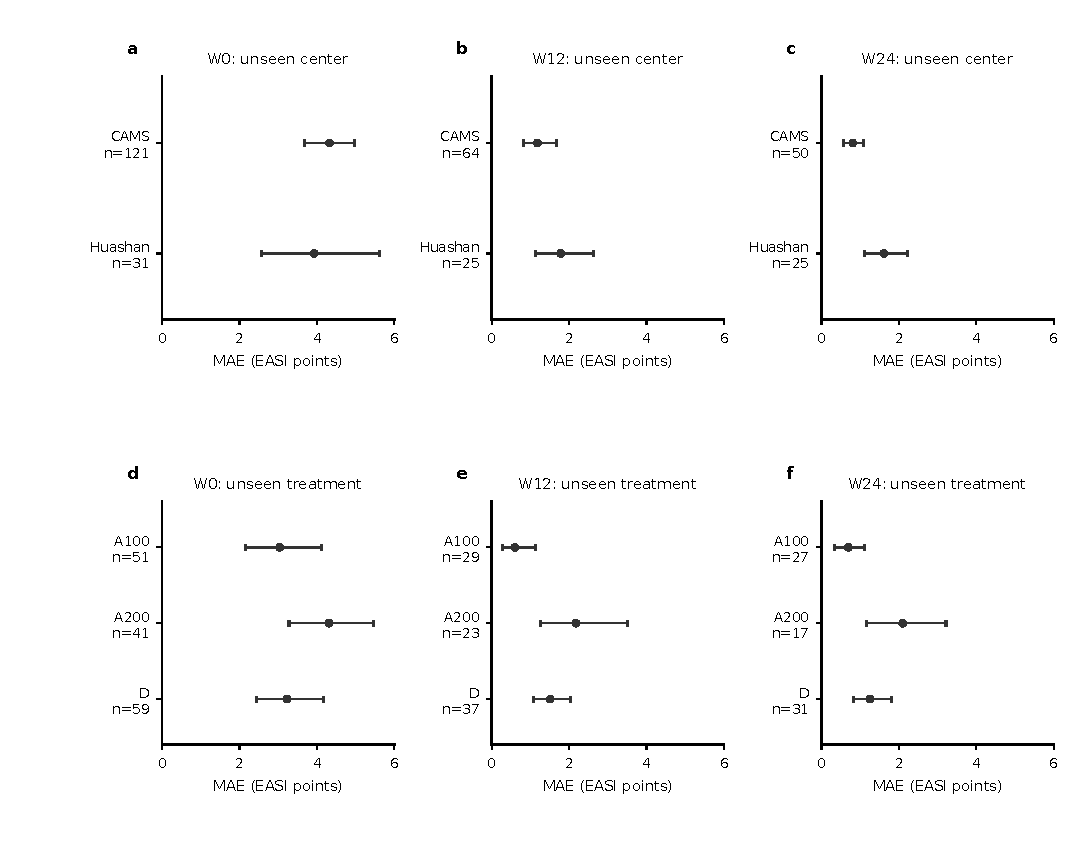
\includegraphics[width=\linewidth,height=.84\textheight,keepaspectratio]{figures/FigureS21.pdf}
\caption{\textbf{Estimation when a centre or treatment group is left out.} Every displayed centre or initial-treatment group was entirely absent from fitting and model-form selection. Points are held-out MAE with patient-bootstrap 95\% confidence intervals; patient counts appear next to each group. The same error scale is used in all panels. These internal transport stress tests are not independent external validation. Sparse groups and different severity distributions affect precision.}\label{fig:FigureS21}
\end{figure}
\clearpage
\renewcommand{\thefigure}{S22}
\begin{figure}[p]
\centering
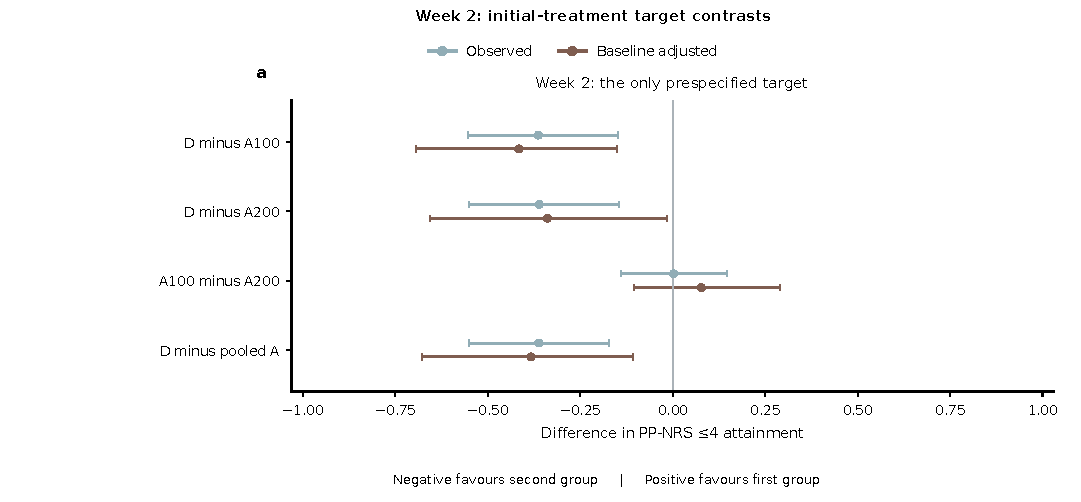
\includegraphics[width=\linewidth,height=.84\textheight,keepaspectratio]{figures/FigureS22.pdf}
\caption{\textbf{Week 2: all initial-treatment target contrasts.} Observed and baseline-adjusted risk differences with nominal 95\% confidence intervals. Positive values favour the first named treatment for target attainment. Adjustment uses generalized overlap weights from baseline EASI, age, sex, BMI and centre; it does not estimate a randomized current-dose effect. D denotes dupilumab; A100/A200 the initial abrocitinib doses. Pooled abrocitinib is supplementary. Missing estimates are left absent; all exact denominators, Fisher/weighted tests, Holm-adjusted P values and exploratory FDR values are in the source tables.}\label{fig:FigureS22}
\end{figure}
\clearpage
\renewcommand{\thefigure}{S23}
\begin{figure}[p]
\centering
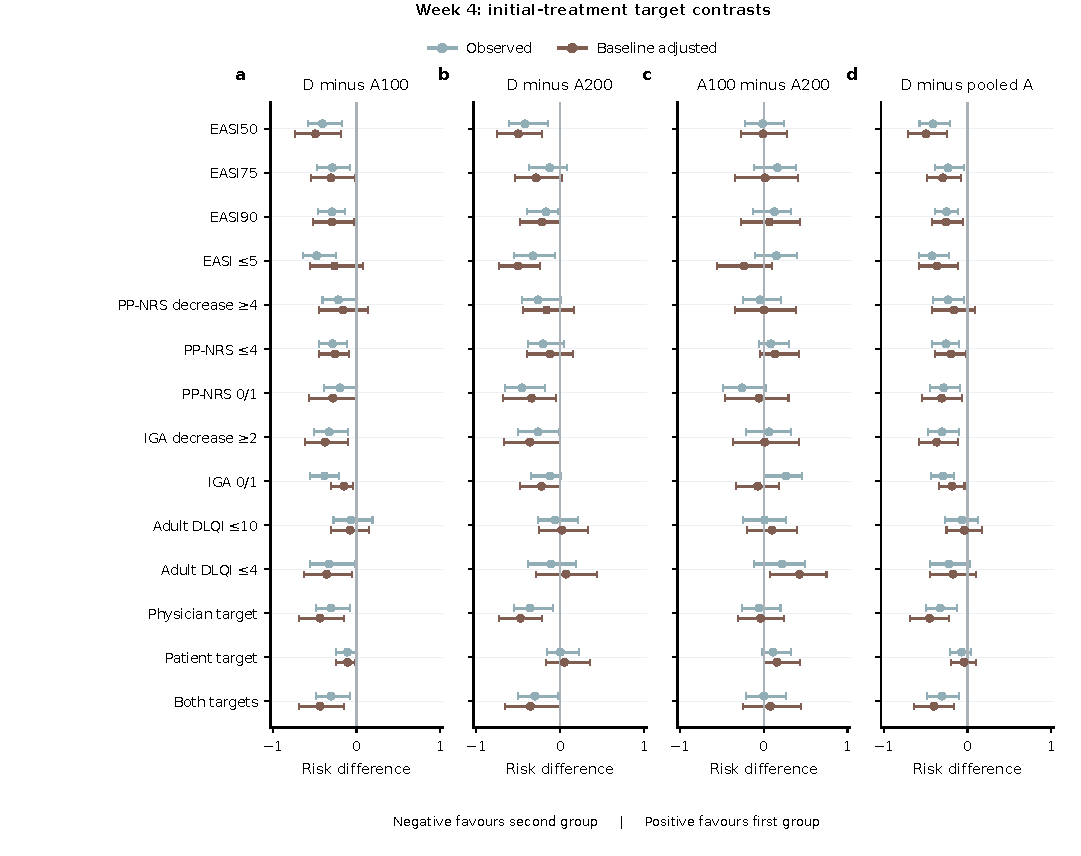
\includegraphics[width=\linewidth,height=.84\textheight,keepaspectratio]{figures/FigureS23.pdf}
\caption{\textbf{Week 4: all initial-treatment target contrasts.} Observed and baseline-adjusted risk differences with nominal 95\% confidence intervals. Positive values favour the first named treatment for target attainment. Adjustment uses generalized overlap weights from baseline EASI, age, sex, BMI and centre; it does not estimate a randomized current-dose effect. D denotes dupilumab; A100/A200 the initial abrocitinib doses. Pooled abrocitinib is supplementary. Missing estimates are left absent; all exact denominators, Fisher/weighted tests, Holm-adjusted P values and exploratory FDR values are in the source tables.}\label{fig:FigureS23}
\end{figure}
\clearpage
\renewcommand{\thefigure}{S24}
\begin{figure}[p]
\centering
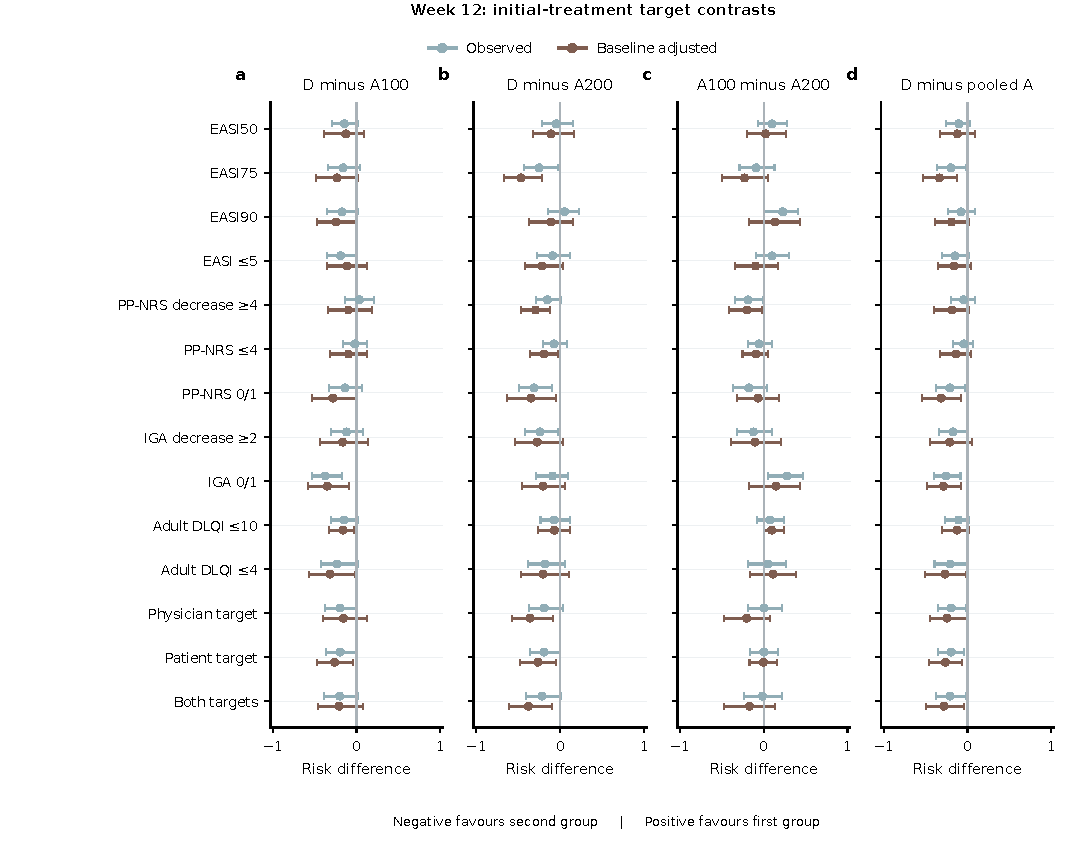
\includegraphics[width=\linewidth,height=.84\textheight,keepaspectratio]{figures/FigureS24.pdf}
\caption{\textbf{Week 12: all initial-treatment target contrasts.} Observed and baseline-adjusted risk differences with nominal 95\% confidence intervals. Positive values favour the first named treatment for target attainment. Adjustment uses generalized overlap weights from baseline EASI, age, sex, BMI and centre; it does not estimate a randomized current-dose effect. D denotes dupilumab; A100/A200 the initial abrocitinib doses. Pooled abrocitinib is supplementary. Missing estimates are left absent; all exact denominators, Fisher/weighted tests, Holm-adjusted P values and exploratory FDR values are in the source tables.}\label{fig:FigureS24}
\end{figure}
\clearpage
\renewcommand{\thefigure}{S25}
\begin{figure}[p]
\centering
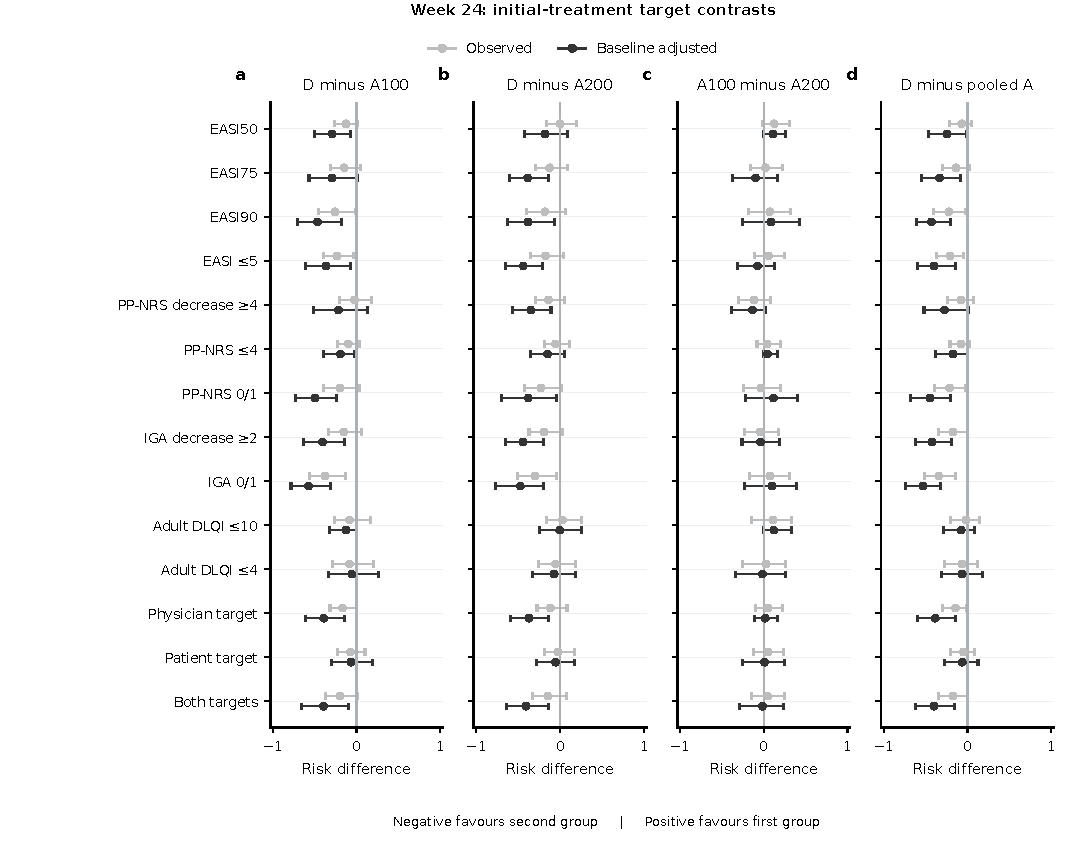
\includegraphics[width=\linewidth,height=.84\textheight,keepaspectratio]{figures/FigureS25.pdf}
\caption{\textbf{Week 24: all initial-treatment target contrasts.} Observed and baseline-adjusted risk differences with nominal 95\% confidence intervals. Positive values favour the first named treatment for target attainment. Adjustment uses generalized overlap weights from baseline EASI, age, sex, BMI and centre; it does not estimate a randomized current-dose effect. D denotes dupilumab; A100/A200 the initial abrocitinib doses. Pooled abrocitinib is supplementary. Missing estimates are left absent; all exact denominators, Fisher/weighted tests, Holm-adjusted P values and exploratory FDR values are in the source tables.}\label{fig:FigureS25}
\end{figure}
\clearpage
\renewcommand{\thefigure}{S26}
\begin{figure}[p]
\centering
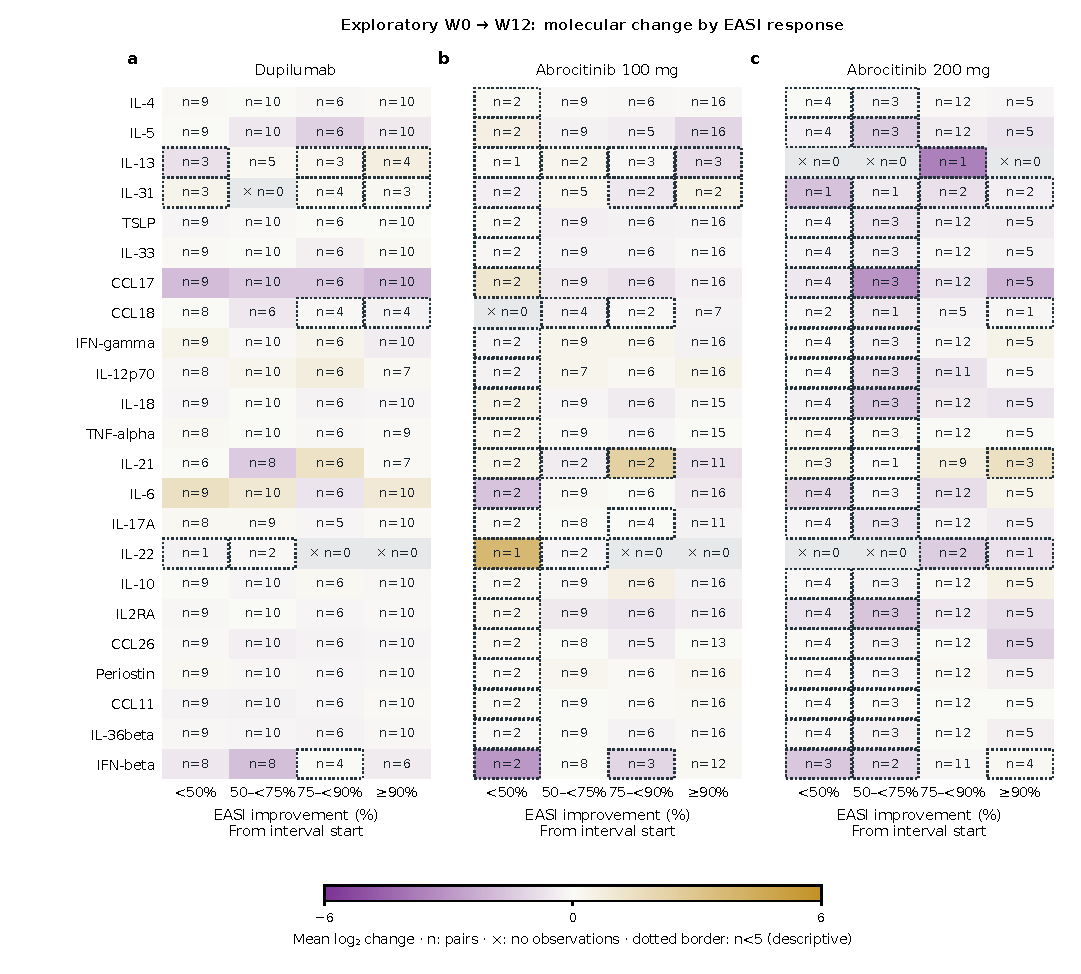
\includegraphics[width=\linewidth,height=.84\textheight,keepaspectratio]{figures/FigureS26.pdf}
\caption{\textbf{Molecular changes by EASI response: W0 $\rightarrow$ W12.} Columns are mutually exclusive clinical-response categories within the named paired interval. Colour is mean within-patient log$_2$ concentration change; numbers are complete-pair patient counts, with a dagger indicating descriptive small cells with n<5. Negative means lower later concentration. These are neither correlation coefficients nor change per clinical point. EASI improvement is relative to the start of the named interval; IGA uses recorded ordinal decrease. Cells marked $\times$ and n=0 have no observations; absence is not a zero molecular change. All 23 markers, exact means and intervals are retained in the source table; the small cells are descriptive and do not validate a prediction model.}\label{fig:FigureS26}
\end{figure}
\clearpage
\renewcommand{\thefigure}{S27}
\begin{figure}[p]
\centering
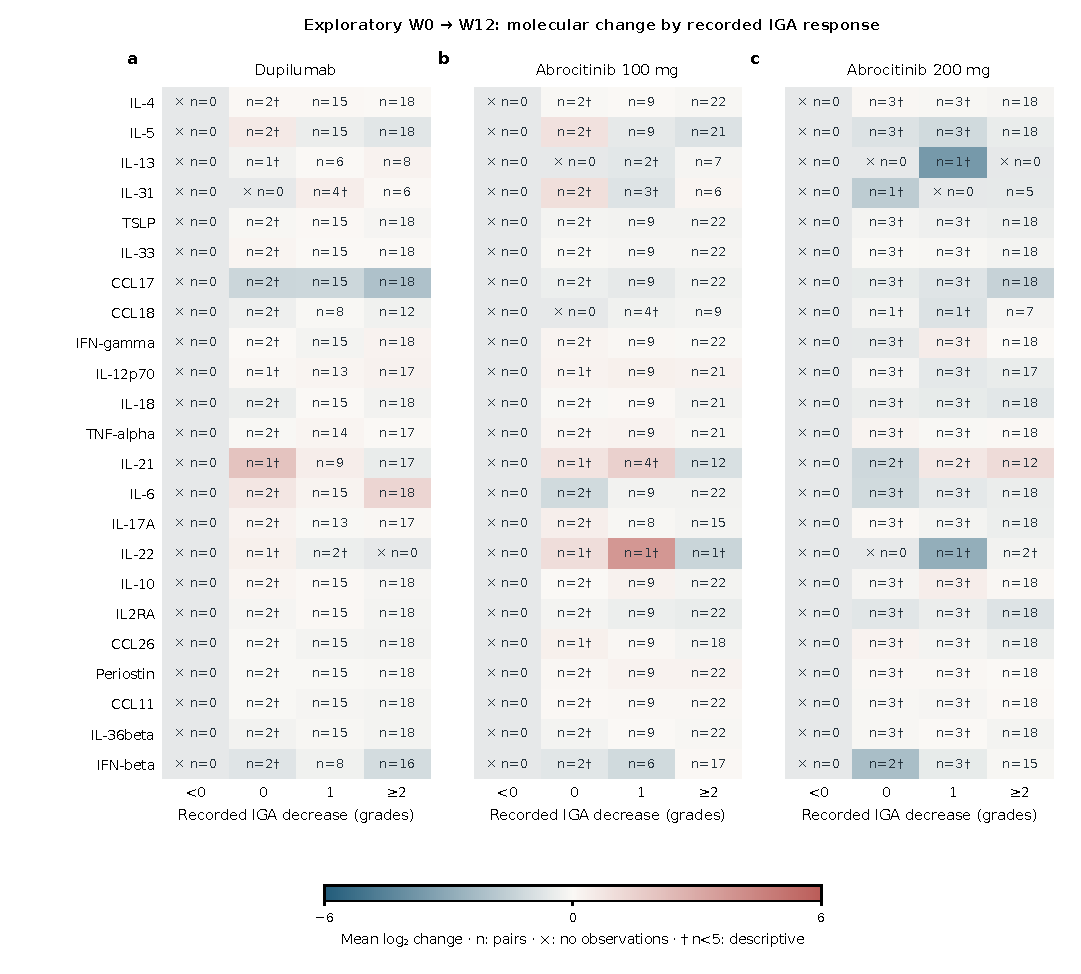
\includegraphics[width=\linewidth,height=.84\textheight,keepaspectratio]{figures/FigureS27.pdf}
\caption{\textbf{Molecular changes by IGA response: W0 $\rightarrow$ W12.} Columns are mutually exclusive clinical-response categories within the named paired interval. Colour is mean within-patient log$_2$ concentration change; numbers are complete-pair patient counts, with a dagger indicating descriptive small cells with n<5. Negative means lower later concentration. These are neither correlation coefficients nor change per clinical point. EASI improvement is relative to the start of the named interval; IGA uses recorded ordinal decrease. Cells marked $\times$ and n=0 have no observations; absence is not a zero molecular change. All 23 markers, exact means and intervals are retained in the source table; the small cells are descriptive and do not validate a prediction model.}\label{fig:FigureS27}
\end{figure}
\clearpage
\renewcommand{\thefigure}{S28}
\begin{figure}[p]
\centering
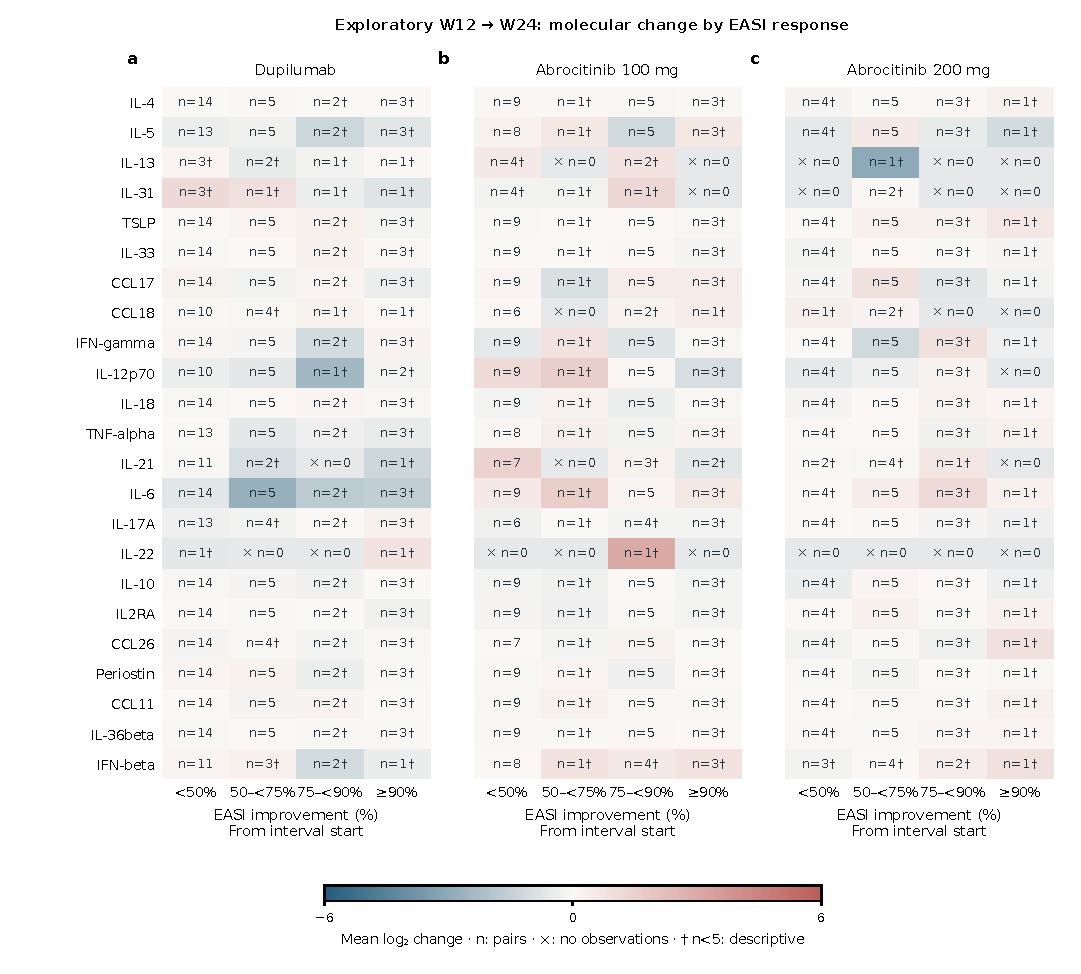
\includegraphics[width=\linewidth,height=.84\textheight,keepaspectratio]{figures/FigureS28.pdf}
\caption{\textbf{Molecular changes by EASI response: W12 $\rightarrow$ W24.} Columns are mutually exclusive clinical-response categories within the named paired interval. Colour is mean within-patient log$_2$ concentration change; numbers are complete-pair patient counts, with a dagger indicating descriptive small cells with n<5. Negative means lower later concentration. These are neither correlation coefficients nor change per clinical point. EASI improvement is relative to the start of the named interval; IGA uses recorded ordinal decrease. Cells marked $\times$ and n=0 have no observations; absence is not a zero molecular change. All 23 markers, exact means and intervals are retained in the source table; the small cells are descriptive and do not validate a prediction model.}\label{fig:FigureS28}
\end{figure}
\clearpage
\renewcommand{\thefigure}{S29}
\begin{figure}[p]
\centering
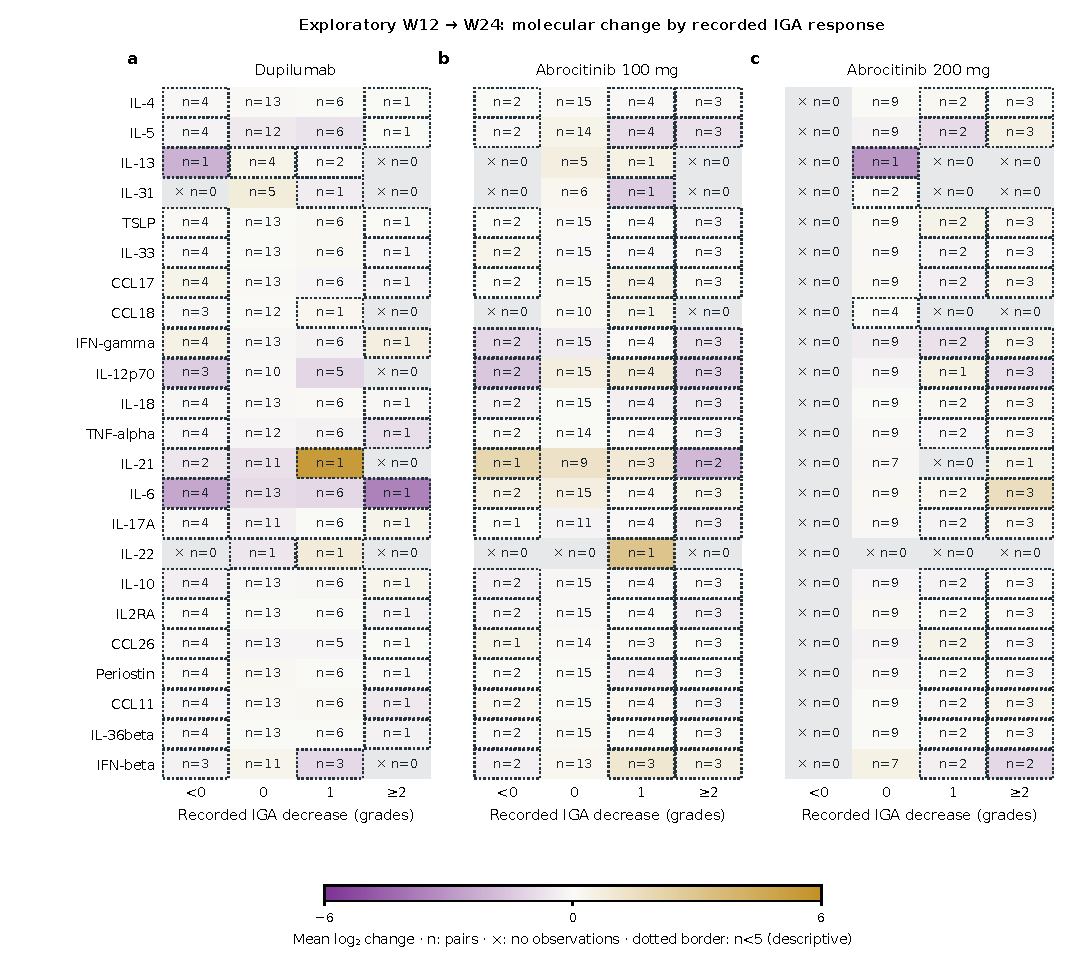
\includegraphics[width=\linewidth,height=.84\textheight,keepaspectratio]{figures/FigureS29.pdf}
\caption{\textbf{Molecular changes by IGA response: W12 $\rightarrow$ W24.} Columns are mutually exclusive clinical-response categories within the named paired interval. Colour is mean within-patient log$_2$ concentration change; numbers are complete-pair patient counts, with a dagger indicating descriptive small cells with n<5. Negative means lower later concentration. These are neither correlation coefficients nor change per clinical point. EASI improvement is relative to the start of the named interval; IGA uses recorded ordinal decrease. Cells marked $\times$ and n=0 have no observations; absence is not a zero molecular change. All 23 markers, exact means and intervals are retained in the source table; the small cells are descriptive and do not validate a prediction model.}\label{fig:FigureS29}
\end{figure}
\clearpage
\renewcommand{\thefigure}{S30}
\begin{figure}[p]
\centering
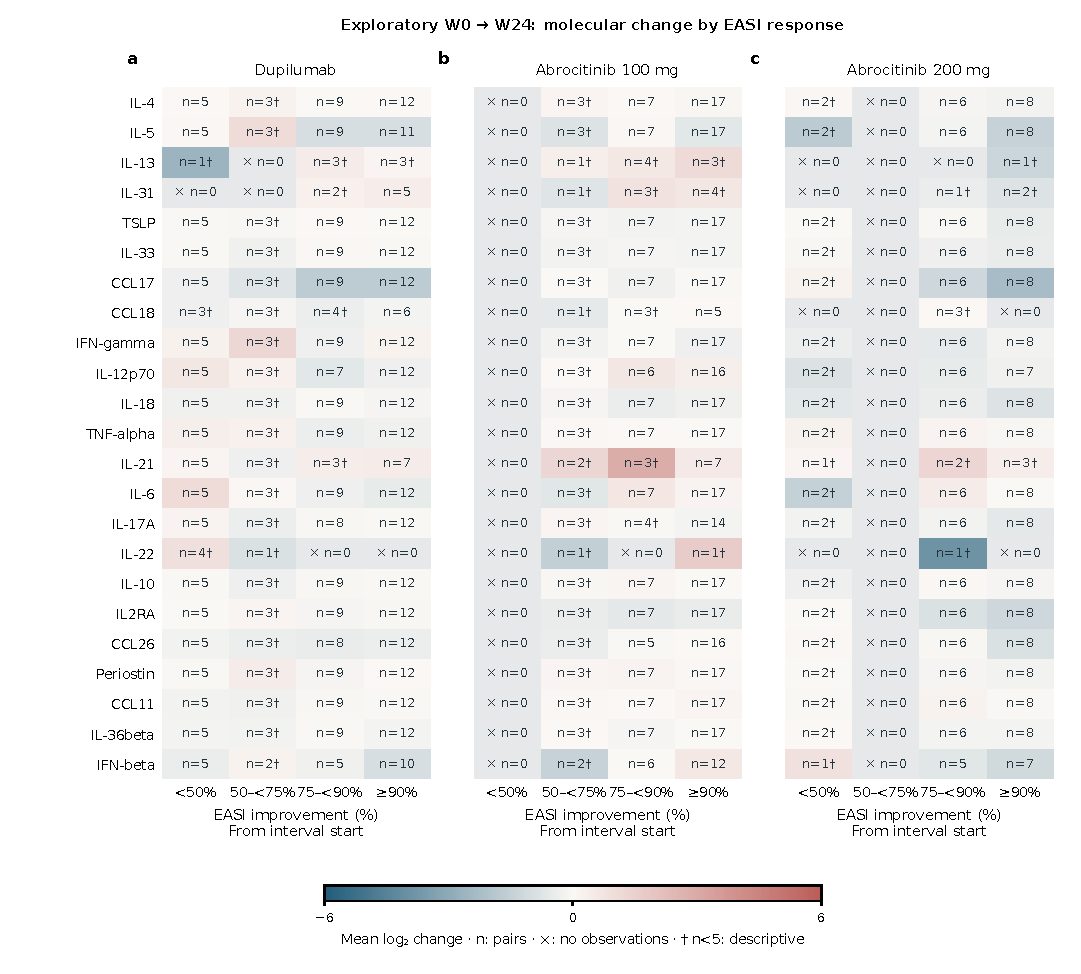
\includegraphics[width=\linewidth,height=.84\textheight,keepaspectratio]{figures/FigureS30.pdf}
\caption{\textbf{Molecular changes by EASI response: W0 $\rightarrow$ W24.} Columns are mutually exclusive clinical-response categories within the named paired interval. Colour is mean within-patient log$_2$ concentration change; numbers are complete-pair patient counts, with a dagger indicating descriptive small cells with n<5. Negative means lower later concentration. These are neither correlation coefficients nor change per clinical point. EASI improvement is relative to the start of the named interval; IGA uses recorded ordinal decrease. Cells marked $\times$ and n=0 have no observations; absence is not a zero molecular change. All 23 markers, exact means and intervals are retained in the source table; the small cells are descriptive and do not validate a prediction model.}\label{fig:FigureS30}
\end{figure}
\clearpage
\renewcommand{\thefigure}{S31}
\begin{figure}[p]
\centering
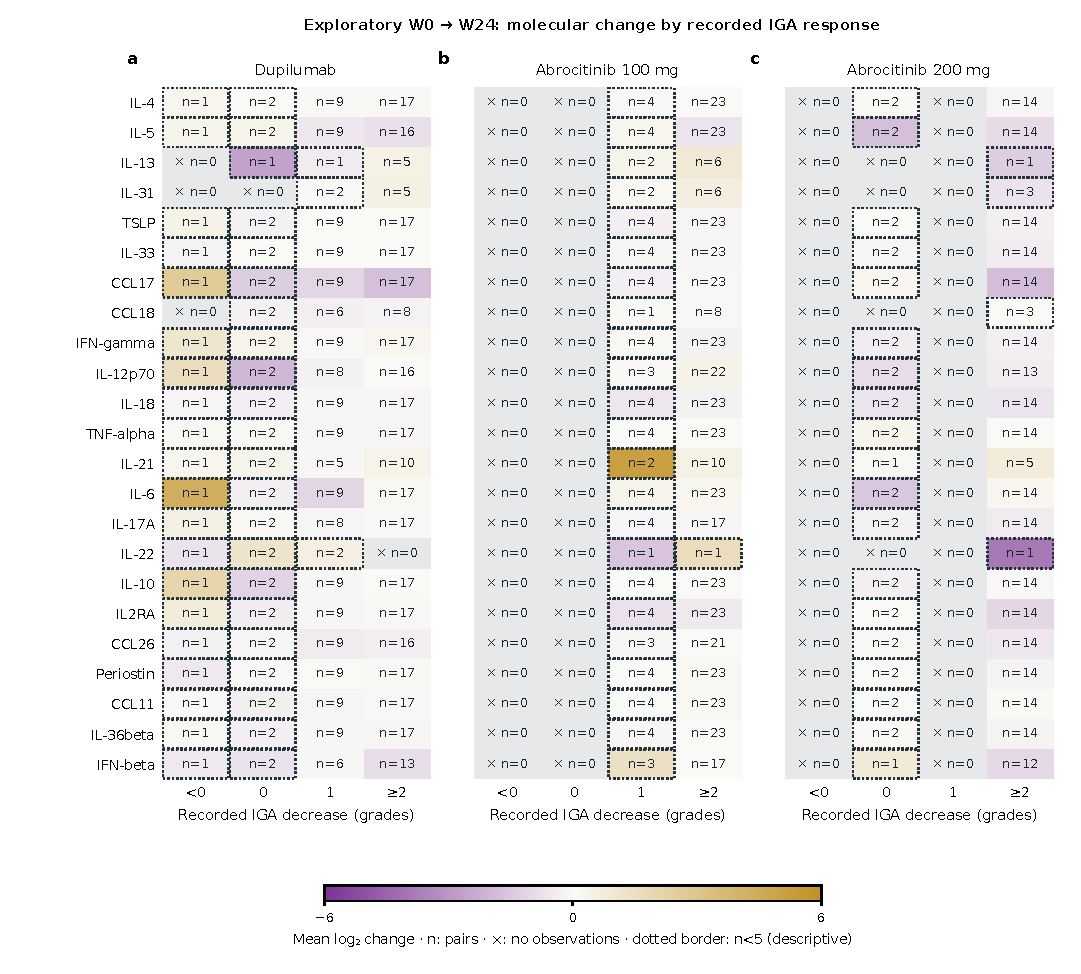
\includegraphics[width=\linewidth,height=.84\textheight,keepaspectratio]{figures/FigureS31.pdf}
\caption{\textbf{Molecular changes by IGA response: W0 $\rightarrow$ W24.} Columns are mutually exclusive clinical-response categories within the named paired interval. Colour is mean within-patient log$_2$ concentration change; numbers are complete-pair patient counts, with a dagger indicating descriptive small cells with n<5. Negative means lower later concentration. These are neither correlation coefficients nor change per clinical point. EASI improvement is relative to the start of the named interval; IGA uses recorded ordinal decrease. Cells marked $\times$ and n=0 have no observations; absence is not a zero molecular change. All 23 markers, exact means and intervals are retained in the source table; the small cells are descriptive and do not validate a prediction model.}\label{fig:FigureS31}
\end{figure}
\clearpage
\renewcommand{\thefigure}{S32}
\begin{figure}[p]
\centering
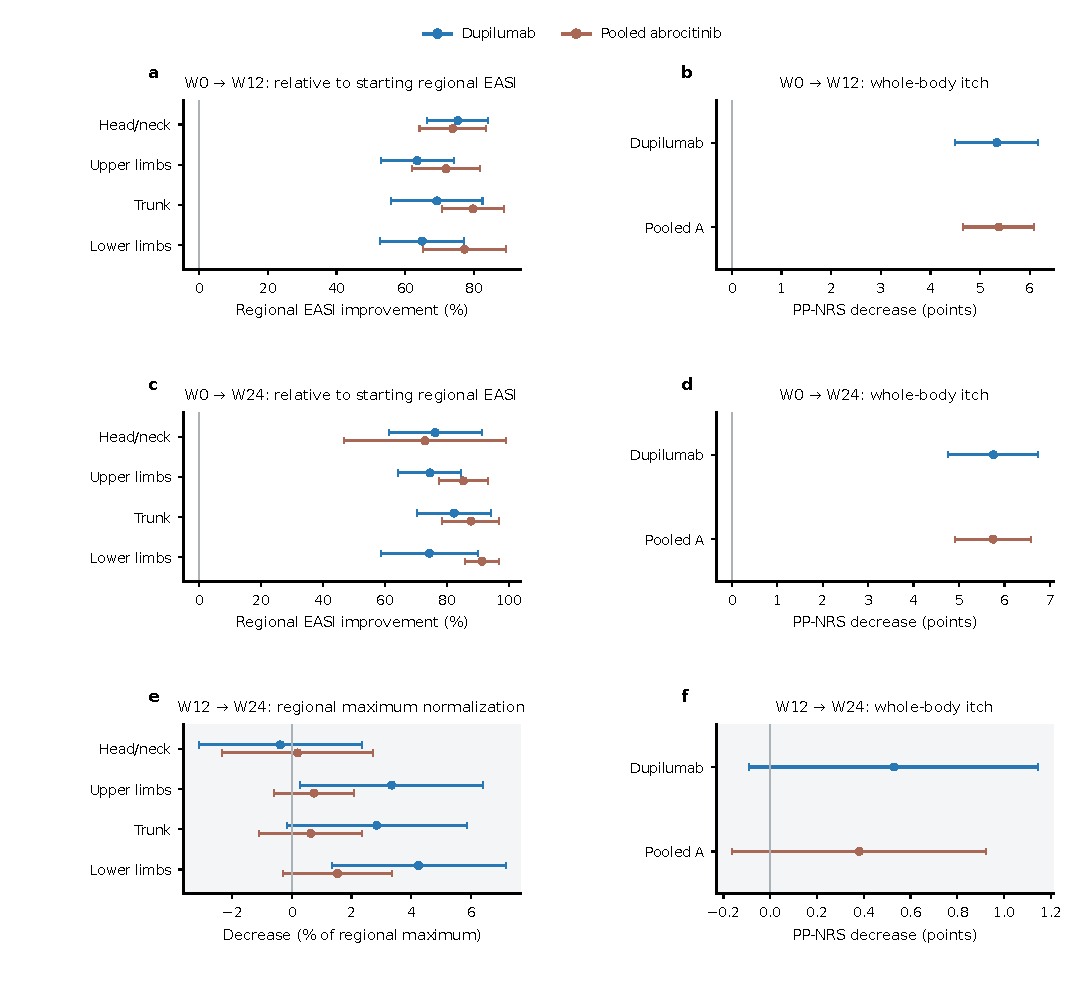
\includegraphics[width=\linewidth,height=.84\textheight,keepaspectratio]{figures/FigureS32.pdf}
\caption{\textbf{Separate paired regional and whole-body itch intervals.} Rows are separate paired intervals that can share patients; they are not a continuous cumulative sequence. First two rows show mean regional percentage improvement relative to positive W0 regional EASI. Last row shows W12$\rightarrow$W24 decrease as a percentage of the regional theoretical maximum, avoiding division by near-zero W12 values. Right, Whole-body PP-NRS decrease in original score points, not regional itch. Positive values indicate improvement, negative worsening. Bars are 95\% t confidence intervals. Source-consistent regional records are required; the separate-dose and adjusted comparisons remain in the tables. No adjusted regional contrast passed the FDR threshold. The pooled abrocitinib group retains its observed dose mixture.}\label{fig:FigureS32}
\end{figure}
\clearpage
\renewcommand{\thefigure}{S33}
\begin{figure}[p]
\centering
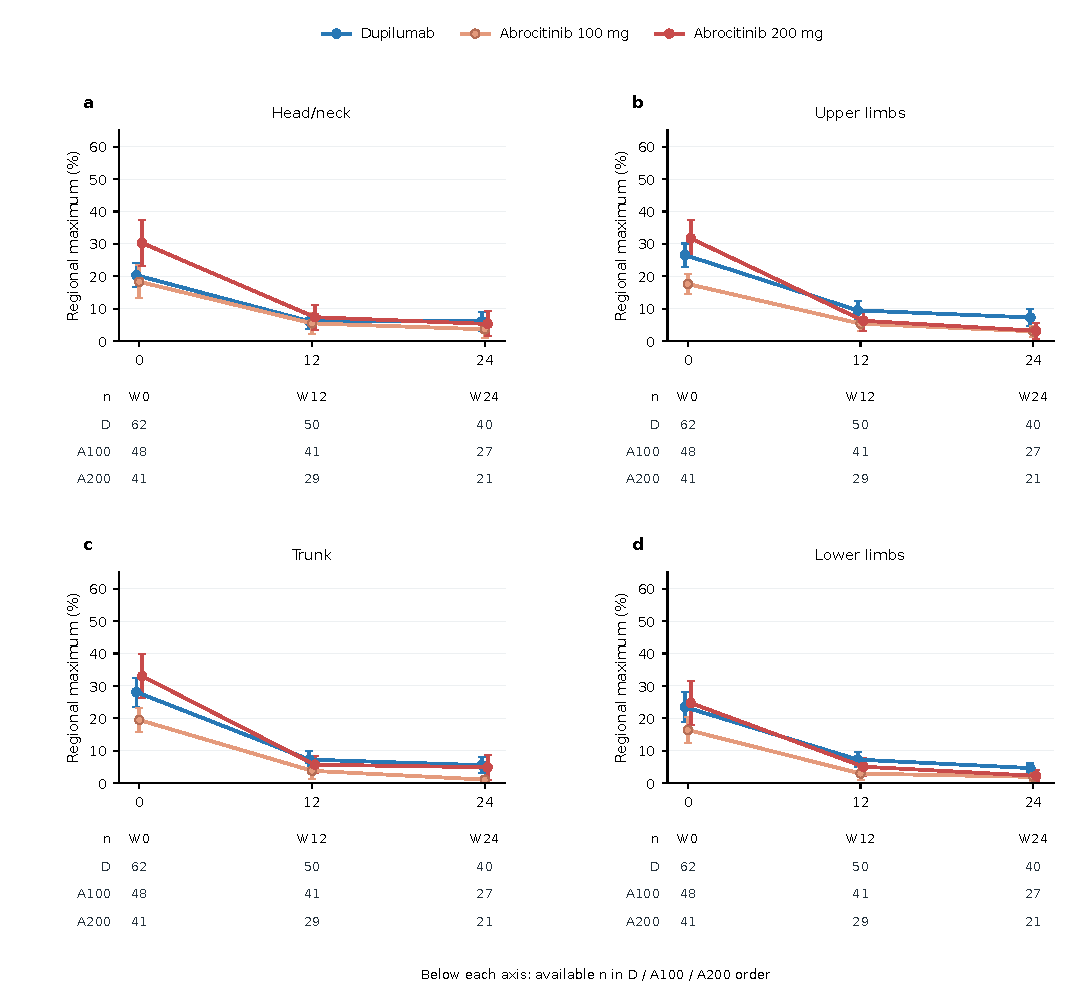
\includegraphics[width=\linewidth,height=.84\textheight,keepaspectratio]{figures/FigureS33.pdf}
\caption{\textbf{Regional burden on a common interpretable scale.} Recorded regional EASI contributions divided by theoretical regional maxima (head/neck 7.2, upper limbs 14.4, trunk 21.6, lower limbs 28.8) and multiplied by 100. Points show observed means and 95\% t confidence intervals, by initial treatment. This rescales skin-region burden; it does not measure molecular inflammation or demonstrate intrinsic anatomical susceptibility. Available patients may differ between visits. Exact n and sensitivity populations accompany the source table.}\label{fig:FigureS33}
\end{figure}
\clearpage
\renewcommand{\thefigure}{S34}
\begin{figure}[p]
\centering
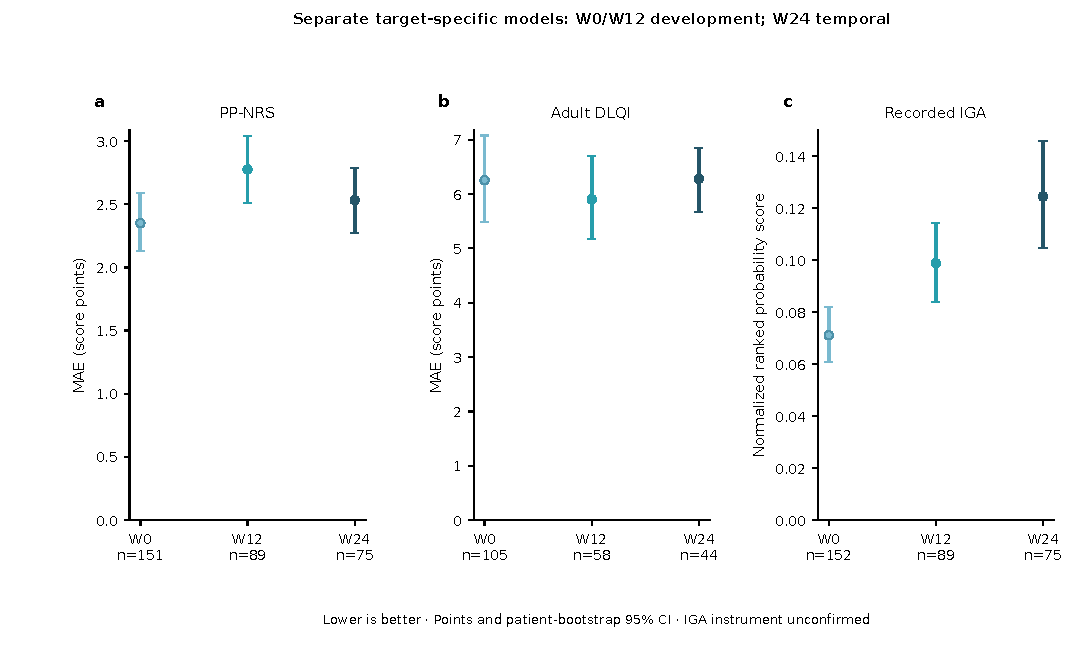
\includegraphics[width=\linewidth,height=.84\textheight,keepaspectratio]{figures/FigureS34.pdf}
\caption{\textbf{Independently fitted PP-NRS, DLQI and ordinal IGA models.} Each target has separate coefficients and patient-grouped nested selection using current BSA and the fixed three-marker panel. PP-NRS and adult DLQI use continuous-outcome models; recorded IGA uses ordinal proportional-odds regression and normalized ranked probability score. Points and patient-bootstrap 95\% confidence intervals show the independently fitted target-specific models; lower is better. W0, W12 and W24 use light blue, teal and deep blue circles. W0/W12 are development visits evaluated in patient-held-out outer folds; W24 is previously inspected same-cohort temporal transfer, not independent external validation. BSA-only controls remain in the numerical source table and are not plotted. No treatment, time label or EASI is used as an input. These results do not establish clinically adequate replacement, and the shared panel is not claimed optimal for every target. Recorded IGA includes grade 5 pending instrument verification.}\label{fig:FigureS34}
\end{figure}
\clearpage
\renewcommand{\thefigure}{S35}
\begin{figure}[p]
\centering
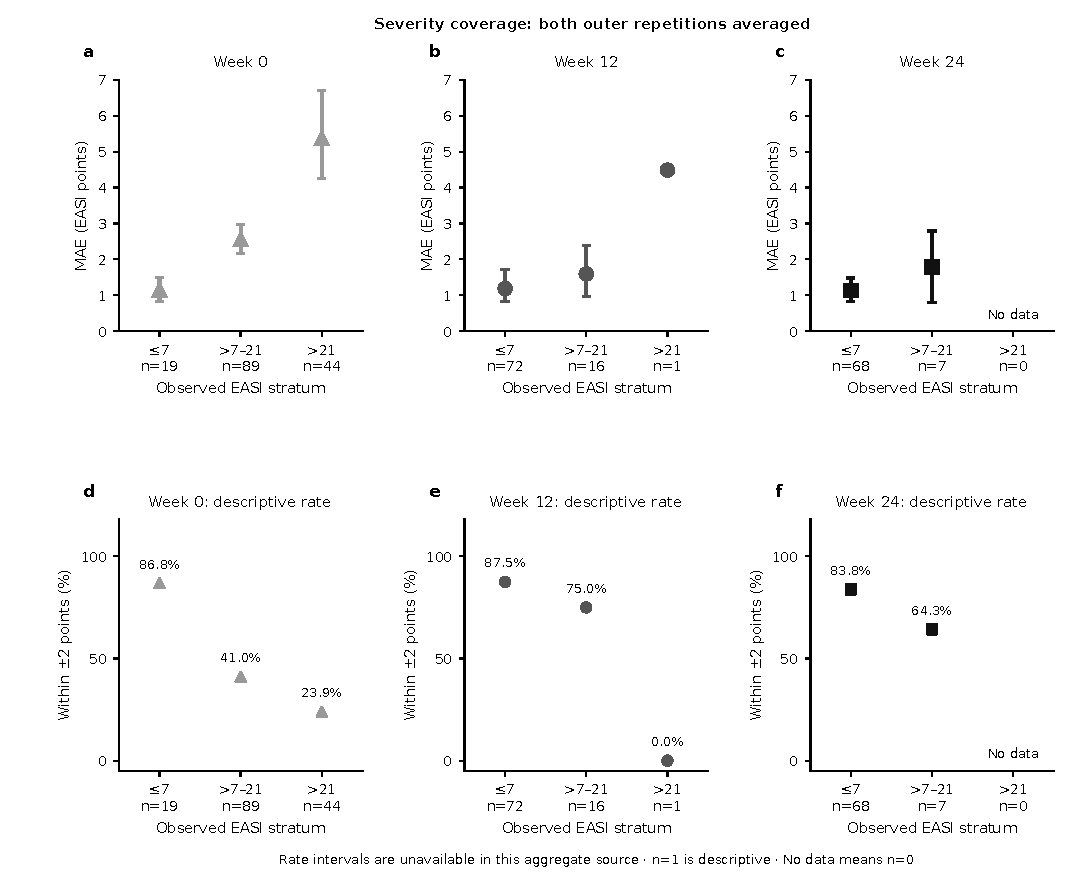
\includegraphics[width=\linewidth,height=.84\textheight,keepaspectratio]{figures/FigureS35.pdf}
\caption{\textbf{Accuracy across observed EASI severity levels.} Primary nested estimator results averaged over both outer repetitions. Top, Mean absolute error and patient-bootstrap 95\% confidence intervals. Bottom, Percentage within two EASI points, with direct values including zero; aggregate-source rate intervals are unavailable and are not fabricated. The n=1 result is descriptive. This is a descriptive accuracy threshold, not established clinical equivalence. Strata use observed EASI for evaluation only, not routing or predictor input. W12 has one severe patient and W24 none, so post-treatment accuracy cannot establish reliable severe-disease performance. Axes retain all interval extents.}\label{fig:FigureS35}
\end{figure}
\clearpage
\renewcommand{\thefigure}{S36}
\begin{figure}[p]
\centering
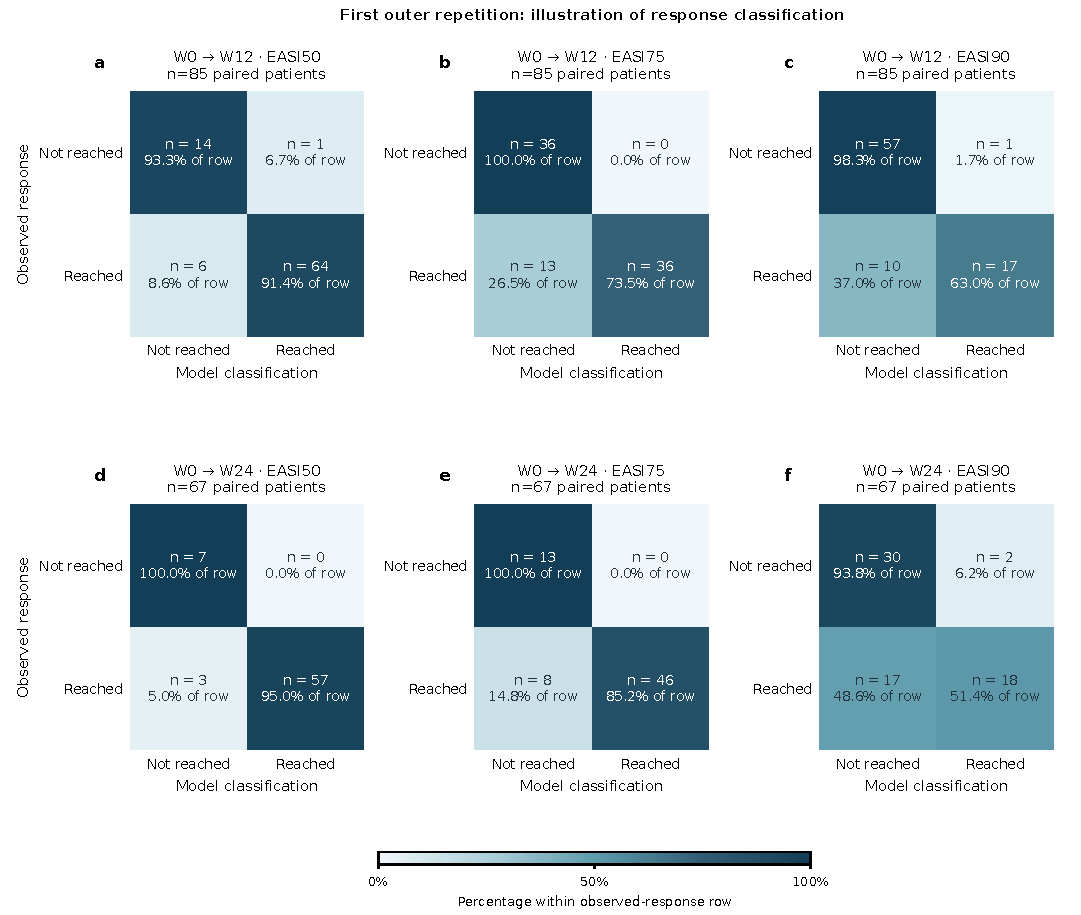
\includegraphics[width=\linewidth,height=.84\textheight,keepaspectratio]{figures/FigureS36.pdf}
\caption{\textbf{Who is correctly classified as reaching EASI50, EASI75 and EASI90?.} Each panel shows actual patient counts from the first outer repetition, separately for W0$\rightarrow$W12 and W0$\rightarrow$W24. Rows are observed response and columns model-estimated response. Diagonal cells are correct; upper-right cells falsely indicate response and lower-left cells miss an observed responder. Percentages are within each observed-response row, so the lower-right percentage is sensitivity and the upper-left percentage specificity. Observed response uses observed baseline/follow-up scores, whereas estimated response uses predicted baseline/follow-up scores. Counts are integers from one repetition, not the primary two-repetition average; the full metrics table retains the latter. The paired denominators are 85 and 67, with no excluded pair for invalid baseline in this displayed repetition. The two intervals can share patients. This assesses response classification, not alternative-treatment outcomes or continuous-score equivalence.}\label{fig:FigureS36}
\end{figure}
\clearpage
\renewcommand{\thefigure}{S37}
\begin{figure}[p]
\centering
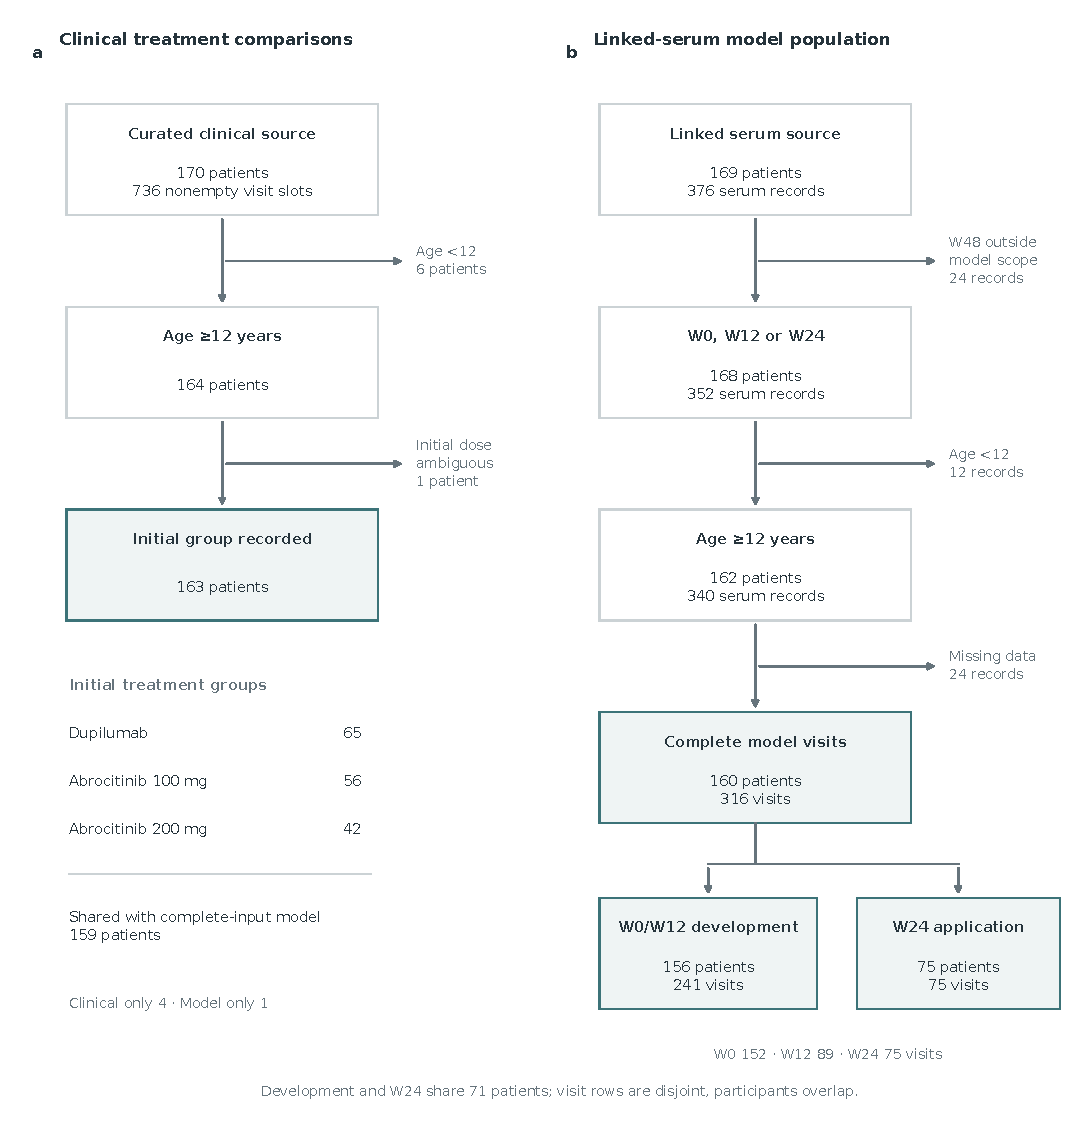
\includegraphics[width=\linewidth,height=.84\textheight,keepaspectratio]{figures/FigureS37.pdf}
\caption{\textbf{Parallel clinical and complete-input model populations.} a, Clinical comparison eligibility starts with 170 curated patients and 1,700 predefined visit slots; 736 slots contain recorded visit data. Six patients aged <12 and one age-eligible patient with an ambiguous initial dose are excluded, leaving 163 patients. This is a record source, not a screened or consented recruitment denominator. b, The linked serum branch is separate and is not a subset of the clinical comparison. Serum records count linked sample rows, not independent participants. Excluding 24 W48 records leaves 168 patients and 352 W0/W12/W24 records; age exclusions remove 12 records from six patients. Complete-case exclusions are sequential and mutually exclusive at the record level. Of the remaining 340 records, 13 lack EASI, one BSA, none CCL17, eight CCL26 and two IL-5, leaving 316 visits from 160 patients. Missing model inputs include unavailable valid positive molecular values. Losing a visit does not necessarily remove the patient. Development comprises 156 patients and 241 visits, W0 n=152 and W12 n=89. W24 comprises 75 patients and 75 visits and is previously inspected within-cohort temporal application, not external validation. The clinical and model populations share 159 patients, with four clinical-only and one model-only. Development and W24 share 71 patients, with 85 development-only and four W24-only. Fifty-one patients have all three complete model visits. Initial-dose ambiguity may remain in the treatment-free model. No missing clinical outcome is filled as validation truth. All exact counts and units remain in the linked flow and overlap source tables.}\label{fig:FigureS37}
\end{figure}
\clearpage
\renewcommand{\thefigure}{S38}
\begin{figure}[p]
\centering
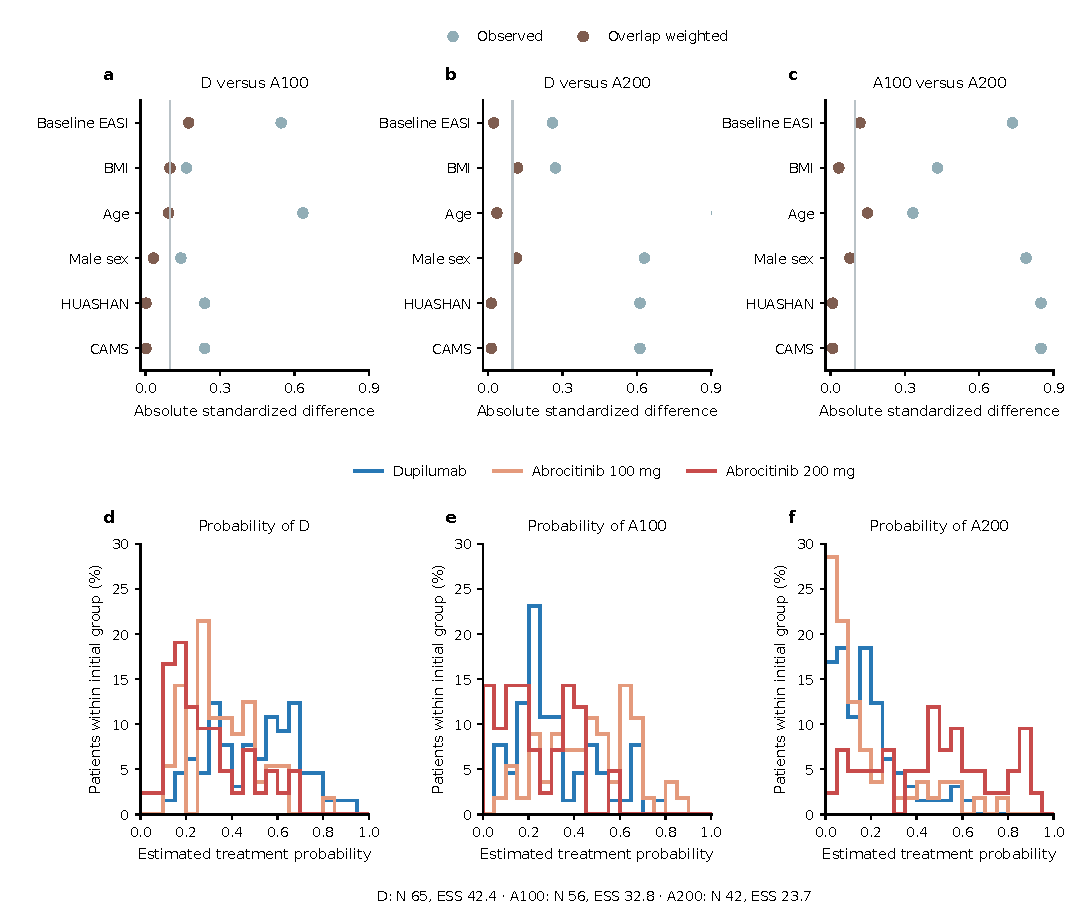
\includegraphics[width=\linewidth,height=.84\textheight,keepaspectratio]{figures/FigureS38.pdf}
\caption{\textbf{Baseline balance, treatment overlap and effective sample size.} a--c, Absolute standardized mean differences for every covariate in the initial-treatment propensity model, before and after generalized overlap weighting. Differences use the unweighted pairwise pooled standard deviation in both displays. The light 0.10 reference line is a descriptive balance guide, not a statistical significance threshold. Residual imbalance remains. d--f, Baseline multinomial treatment probabilities, stratified by actual initial treatment; each distribution uses all patients in that initial group and sums to 100\%. These show common support rather than longitudinal drug exposure. The footer reports original N and effective sample size, (sum w)$^2$/sum(w$^2$). All centre, sex, age, BMI and EASI variables are shown. Overlap weighting targets comparable baseline patients; it cannot remove unmeasured confounding or correct outcome-driven dose changes. Endpoint- and marker-specific availability/ESS diagnostics are retained in the source tables.}\label{fig:FigureS38}
\end{figure}
\clearpage
\renewcommand{\thefigure}{S39}
\begin{figure}[p]
\centering
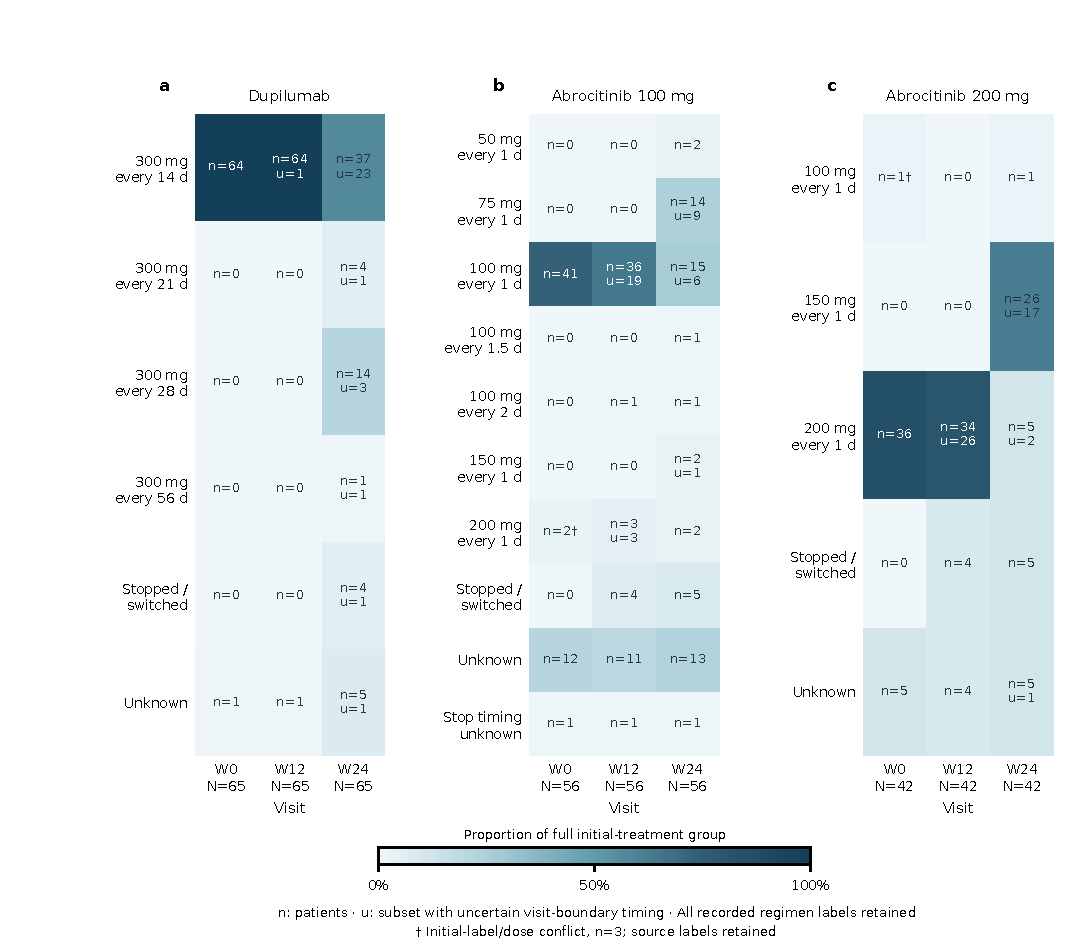
\includegraphics[width=\linewidth,height=.84\textheight,keepaspectratio]{figures/FigureS39.pdf}
\caption{\textbf{Recorded regimens evolve after the initial treatment assignment.} Within each initial-treatment group, the table-like heatmap shows all recorded regimens at W0/W12/W24. Cell n values are patient counts; u denotes the subset with uncertain timing relative to the visit boundary. Blue intensity is the proportion of the full initial-treatment group, with a fixed 0--100\% scale. Zero cells are genuine zero counts. Unknown regimens, uncertain stop timing and stopping/switching are retained; all 163 patients remain represented. W0 is the recorded starting regimen and must not be read as prior systemic exposure. Daggers flag three unresolved source conflicts at W0: two patients assigned to the initial A100 source group have a recorded 200 mg regimen and one assigned to A200 has a recorded 100 mg regimen. The source group and recorded regimen are both preserved; these are not presumed switches. Recorded 75 mg and 150 mg labels are preserved without assuming that they mean alternate-day 100 mg or 200 mg. This aggregate display is not an individual transition flow and does not resolve whether a treatment decision preceded or followed the outcome assessment.}\label{fig:FigureS39}
\end{figure}
\clearpage
\renewcommand{\thefigure}{S40}
\begin{figure}[p]
\centering
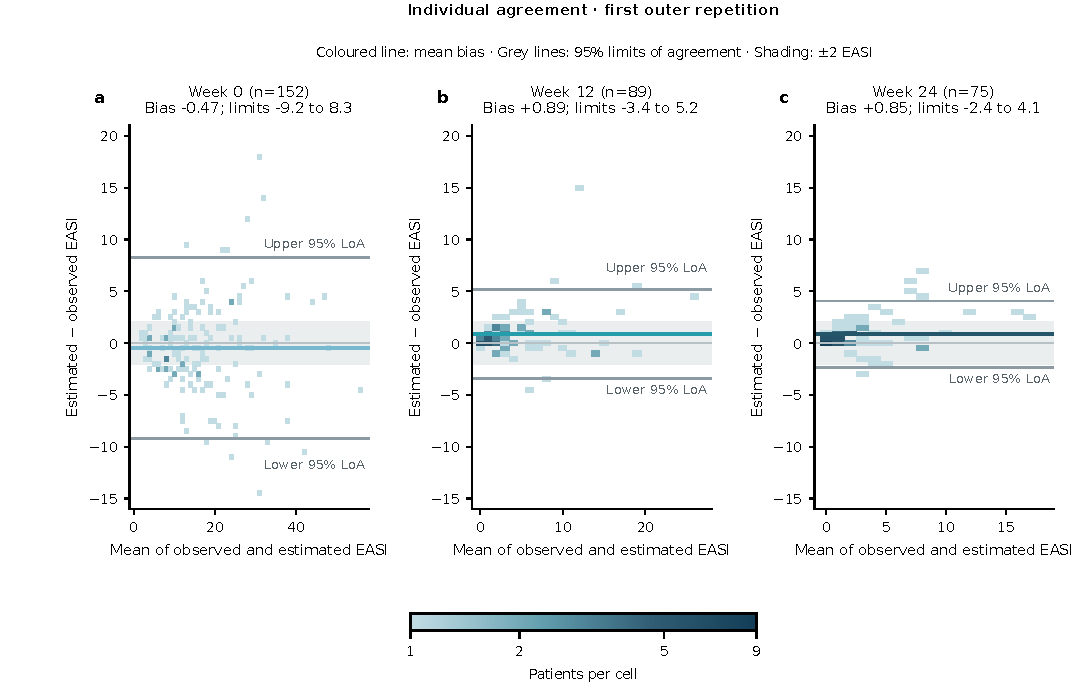
\includegraphics[width=\linewidth,height=.84\textheight,keepaspectratio]{figures/FigureS40.pdf}
\caption{\textbf{Individual agreement across the range of EASI.} Bland--Altman count maps from the first outer repetition. Each equal-size cell spans one EASI point horizontally and half a point vertically; colour gives patient count on the labelled logarithmic scale. All 152/89/75 patients at W0/W12/W24 are retained. The vertical axis is estimated minus observed EASI; negative values indicate underestimation. Coloured horizontal lines show mean bias. Grey labelled lines are 95\% limits of agreement (mean bias $\pm$1.96 error SD), not confidence intervals. The common vertical scale contains every error and both limits. The $\pm$2-point shaded band is a reading guide, not a validated equivalence margin. W0/W12 predictions are patient-held-out; W24 is same-cohort temporal application. Table 2 gives primary metrics averaged after scoring both repetitions.}\label{fig:FigureS40}
\end{figure}
\clearpage
\renewcommand{\thefigure}{S41}
\begin{figure}[p]
\centering
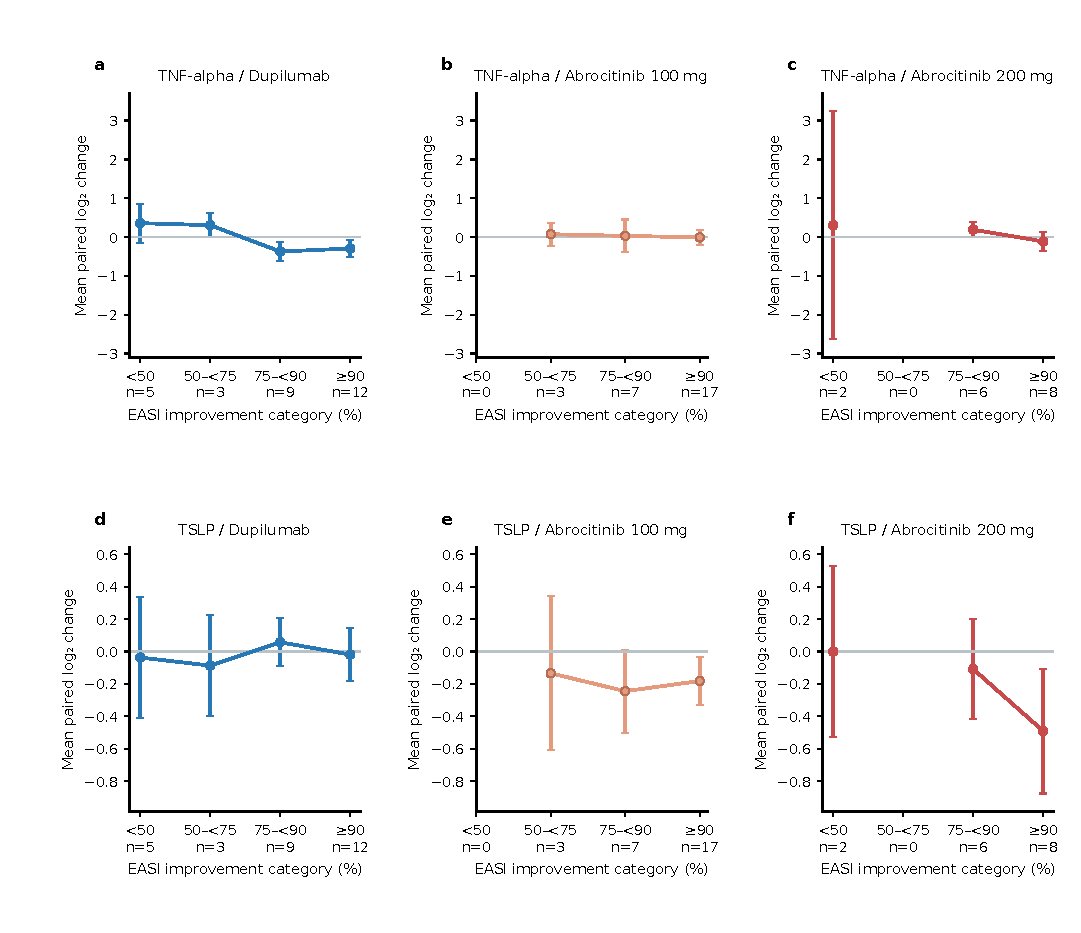
\includegraphics[width=\linewidth,height=.84\textheight,keepaspectratio]{figures/FigureS41.pdf}
\caption{\textbf{EASI-associated molecular changes across response depth.} Exploratory descriptive plots for every marker whose change--EASI association met q<0.05 in the complete molecular--clinical test family (23 markers, five outcomes, three treatments and three windows). Both selected markers arise from W0--W24. Selection used the association family, not tests performed on these categories. All three initial treatments are shown. Points and available 95\% t intervals summarize within-patient log$_2$ concentration changes in mutually exclusive observed EASI-improvement categories; counts are printed below each category. Connecting lines join ordered categories, not visits. Sparse groups with fewer than five pairs are descriptive; absent intervals are not fabricated. The source tables retain all associations, including non-significant results. These same-data descriptions are not independent validation.}\label{fig:FigureS41}
\end{figure}
\end{document}
